% random seed used: 42
\mcglobalheader
\def\mcserialnumber{10}
\mcpaperheader


\def\mcquestionnumber{1}


\mcquestionheader Come si chiama il satellite naturale della Terra?\\
{$A$}: Sole\ \ {$B$}: ISS\ \ {$C$}: Marte\ \ {$D$}: Luna\ \ 

\mcquestionfooter



\def\mcquestionnumber{2}


\mcquestionheader In quale anno il COVID ha fatto la sua comparsa?\\
{$A$}: 2020\ \ {$B$}: 2019\ \ {$C$}: 2001\ \ {$D$}: 1943\ \ 

\mcquestionfooter



\def\mcquestionnumber{3}


\mcquestionheader Dato il vettore $\vec{d}$ in figura, determina il modulo e la componente $d_x$: \begin{figure}[h!]   \begin{center}     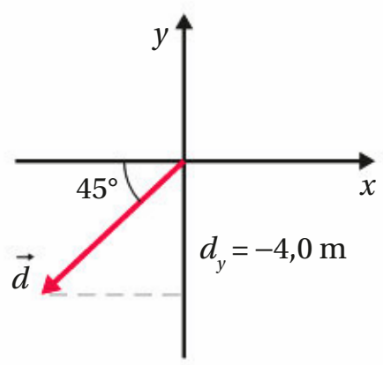
\includegraphics[scale=0.35]{vettored.png}   \end{center} \end{figure}\\
{$A$}: -5,7 m; 4,0 m\ \ {$B$}: 5,7 m; -4,0 m\ \ {$C$}: -5,7 m; -4,0 m\ \ {$D$}: 5,7 m; 4,0 m\ \ 

\mcquestionfooter



\def\mcquestionnumber{4}


\mcquestionheader Il modulo del vettore $\vec{A}(2;2)$ è\\
{$A$}: non so\ \ {$B$}: boh\ \ {$C$}: chissà\ \ 

\mcquestionfooter



\def\mcquestionnumber{5}


\mcquestionheader Raddoppiando la distanza tra due cariche elettriche puntiformi, la forza elettrostatica diminuisce del\\
{$A$}: 50\%\ \ {$B$}: 75\%\ \ {$C$}: 25\%\ \ {$D$}: 90\%\ \ 

\mcquestionfooter



\def\mcquestionnumber{6}


\mcquestionheader In che anno pare sia nato Gesù?\\
{$A$}: 20\ \ {$B$}: 2019\ \ {$C$}: -80\ \ {$D$}: 0\ \ 

\mcquestionfooter



\def\mcquestionnumber{7}


\mcquestionheader Di che colore era il cavallo bianco di Napoleone?\\
{$A$}: Blu\ \ {$B$}: Marrone\ \ {$C$}: Verde\ \ {$D$}: Bianco\ \ 

\mcquestionfooter



\def\mcquestionnumber{8}


\mcquestionheader Qual è la capitale d’Italia?\\
{$A$}: Milano\ \ {$B$}: Roma\ \ {$C$}: Berlino\ \ {$D$}: Parigi\ \ 

\mcquestionfooter



\def\mcquestionnumber{9}


\mcquestionheader Se mischio blu e giallo che colore ottengo?\\
{$A$}: Giallu\ \ {$B$}: Rosso\ \ {$C$}: Verde\ \ {$D$}: Blallo\ \ 

\mcquestionfooter



\def\mcquestionnumber{10}


\mcquestionheader I due vettori $\vec{a}$ e $\vec{b}$ hanno lo stesso modulo e la stessa direzione. Quale delle seguenti affermazioni è falsa?\\
{$A$}: I due vettori sono sicuramente uguali\ \ {$B$}: Tutte le altre\ \ {$C$}: La loro somma è sicuramente nulla\ \ {$D$}: La loro somma non può mai essere zero\ \ 

\mcquestionfooter



\def\mcquestionnumber{11}


\mcquestionheader Seguendo la mappa di un tesoro, un pirata cammina per 2,00~km verso nord-est, poi per 5,00~km verso est, quindi per 2,00~km verso sud-est e infine per 3,00~km verso ovest. Arrivato alla fine del percorso a che distanza si trova dalla posizione che occupava alla partenza?\\
{$A$}: 4,76 km\ \ {$B$}: 4,83 km\ \ {$C$}: 6,32 km\ \ {$D$}: 4,59 km\ \ 

\mcquestionfooter



\def\mcquestionnumber{12}


\mcquestionheader Un gatto percorre 90,0~m verso sud e poi prosegue per altri 120~m verso ovest. Lo spostamento e la distanza percorsa sono rispettivamente\\
{$A$}: 150~m e 210~m\ \ {$B$}: 210~m e 210~m\ \ {$C$}: 210~m e 150~m\ \ {$D$}: 30~m e 210~m\ \ 

\mcquestionfooter



\mcpaperfooter

\def\mcserialnumber{11}
\mcpaperheader


\def\mcquestionnumber{1}


\mcquestionheader Se mischio blu e giallo che colore ottengo?\\
{$A$}: Giallu\ \ {$B$}: Blallo\ \ {$C$}: Verde\ \ {$D$}: Rosso\ \ 

\mcquestionfooter



\def\mcquestionnumber{2}


\mcquestionheader Di che colore era il cavallo bianco di Napoleone?\\
{$A$}: Verde\ \ {$B$}: Marrone\ \ {$C$}: Bianco\ \ {$D$}: Blu\ \ 

\mcquestionfooter



\def\mcquestionnumber{3}


\mcquestionheader Raddoppiando la distanza tra due cariche elettriche puntiformi, la forza elettrostatica diminuisce del\\
{$A$}: 75\%\ \ {$B$}: 25\%\ \ {$C$}: 50\%\ \ {$D$}: 90\%\ \ 

\mcquestionfooter



\def\mcquestionnumber{4}


\mcquestionheader In quale anno il COVID ha fatto la sua comparsa?\\
{$A$}: 2001\ \ {$B$}: 1943\ \ {$C$}: 2019\ \ {$D$}: 2020\ \ 

\mcquestionfooter



\def\mcquestionnumber{5}


\mcquestionheader Come si chiama il satellite naturale della Terra?\\
{$A$}: Marte\ \ {$B$}: Sole\ \ {$C$}: Luna\ \ {$D$}: ISS\ \ 

\mcquestionfooter



\def\mcquestionnumber{6}


\mcquestionheader Il modulo del vettore $\vec{A}(2;2)$ è\\
{$A$}: boh\ \ {$B$}: chissà\ \ {$C$}: non so\ \ 

\mcquestionfooter



\def\mcquestionnumber{7}


\mcquestionheader In che anno pare sia nato Gesù?\\
{$A$}: -80\ \ {$B$}: 2019\ \ {$C$}: 0\ \ {$D$}: 20\ \ 

\mcquestionfooter



\def\mcquestionnumber{8}


\mcquestionheader Seguendo la mappa di un tesoro, un pirata cammina per 2,00~km verso nord-est, poi per 5,00~km verso est, quindi per 2,00~km verso sud-est e infine per 3,00~km verso ovest. Arrivato alla fine del percorso a che distanza si trova dalla posizione che occupava alla partenza?\\
{$A$}: 4,83 km\ \ {$B$}: 4,59 km\ \ {$C$}: 6,32 km\ \ {$D$}: 4,76 km\ \ 

\mcquestionfooter



\def\mcquestionnumber{9}


\mcquestionheader Un gatto percorre 90,0~m verso sud e poi prosegue per altri 120~m verso ovest. Lo spostamento e la distanza percorsa sono rispettivamente\\
{$A$}: 150~m e 210~m\ \ {$B$}: 210~m e 210~m\ \ {$C$}: 30~m e 210~m\ \ {$D$}: 210~m e 150~m\ \ 

\mcquestionfooter



\def\mcquestionnumber{10}


\mcquestionheader Dato il vettore $\vec{d}$ in figura, determina il modulo e la componente $d_x$: \begin{figure}[h!]   \begin{center}     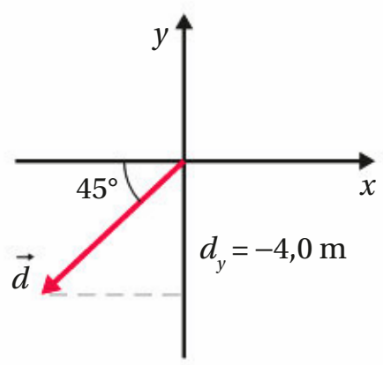
\includegraphics[scale=0.35]{vettored.png}   \end{center} \end{figure}\\
{$A$}: -5,7 m; 4,0 m\ \ {$B$}: -5,7 m; -4,0 m\ \ {$C$}: 5,7 m; -4,0 m\ \ {$D$}: 5,7 m; 4,0 m\ \ 

\mcquestionfooter



\def\mcquestionnumber{11}


\mcquestionheader Qual è la capitale d’Italia?\\
{$A$}: Milano\ \ {$B$}: Roma\ \ {$C$}: Berlino\ \ {$D$}: Parigi\ \ 

\mcquestionfooter



\def\mcquestionnumber{12}


\mcquestionheader I due vettori $\vec{a}$ e $\vec{b}$ hanno lo stesso modulo e la stessa direzione. Quale delle seguenti affermazioni è falsa?\\
{$A$}: La loro somma è sicuramente nulla\ \ {$B$}: La loro somma non può mai essere zero\ \ {$C$}: Tutte le altre\ \ {$D$}: I due vettori sono sicuramente uguali\ \ 

\mcquestionfooter



\mcpaperfooter

\def\mcserialnumber{12}
\mcpaperheader


\def\mcquestionnumber{1}


\mcquestionheader Di che colore era il cavallo bianco di Napoleone?\\
{$A$}: Bianco\ \ {$B$}: Blu\ \ {$C$}: Marrone\ \ {$D$}: Verde\ \ 

\mcquestionfooter



\def\mcquestionnumber{2}


\mcquestionheader Qual è la capitale d’Italia?\\
{$A$}: Roma\ \ {$B$}: Berlino\ \ {$C$}: Parigi\ \ {$D$}: Milano\ \ 

\mcquestionfooter



\def\mcquestionnumber{3}


\mcquestionheader Se mischio blu e giallo che colore ottengo?\\
{$A$}: Giallu\ \ {$B$}: Verde\ \ {$C$}: Rosso\ \ {$D$}: Blallo\ \ 

\mcquestionfooter



\def\mcquestionnumber{4}


\mcquestionheader Raddoppiando la distanza tra due cariche elettriche puntiformi, la forza elettrostatica diminuisce del\\
{$A$}: 90\%\ \ {$B$}: 50\%\ \ {$C$}: 25\%\ \ {$D$}: 75\%\ \ 

\mcquestionfooter



\def\mcquestionnumber{5}


\mcquestionheader Un gatto percorre 90,0~m verso sud e poi prosegue per altri 120~m verso ovest. Lo spostamento e la distanza percorsa sono rispettivamente\\
{$A$}: 30~m e 210~m\ \ {$B$}: 210~m e 210~m\ \ {$C$}: 210~m e 150~m\ \ {$D$}: 150~m e 210~m\ \ 

\mcquestionfooter



\def\mcquestionnumber{6}


\mcquestionheader In quale anno il COVID ha fatto la sua comparsa?\\
{$A$}: 2001\ \ {$B$}: 2020\ \ {$C$}: 1943\ \ {$D$}: 2019\ \ 

\mcquestionfooter



\def\mcquestionnumber{7}


\mcquestionheader In che anno pare sia nato Gesù?\\
{$A$}: 0\ \ {$B$}: -80\ \ {$C$}: 20\ \ {$D$}: 2019\ \ 

\mcquestionfooter



\def\mcquestionnumber{8}


\mcquestionheader Come si chiama il satellite naturale della Terra?\\
{$A$}: Luna\ \ {$B$}: Sole\ \ {$C$}: ISS\ \ {$D$}: Marte\ \ 

\mcquestionfooter



\def\mcquestionnumber{9}


\mcquestionheader Seguendo la mappa di un tesoro, un pirata cammina per 2,00~km verso nord-est, poi per 5,00~km verso est, quindi per 2,00~km verso sud-est e infine per 3,00~km verso ovest. Arrivato alla fine del percorso a che distanza si trova dalla posizione che occupava alla partenza?\\
{$A$}: 4,59 km\ \ {$B$}: 4,83 km\ \ {$C$}: 6,32 km\ \ {$D$}: 4,76 km\ \ 

\mcquestionfooter



\def\mcquestionnumber{10}


\mcquestionheader Dato il vettore $\vec{d}$ in figura, determina il modulo e la componente $d_x$: \begin{figure}[h!]   \begin{center}     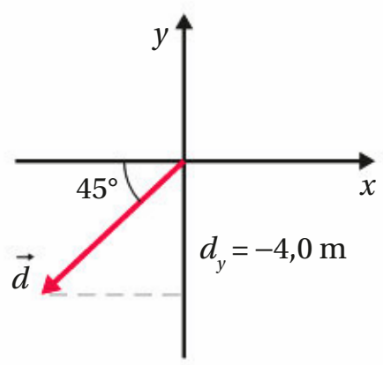
\includegraphics[scale=0.35]{vettored.png}   \end{center} \end{figure}\\
{$A$}: -5,7 m; 4,0 m\ \ {$B$}: 5,7 m; 4,0 m\ \ {$C$}: 5,7 m; -4,0 m\ \ {$D$}: -5,7 m; -4,0 m\ \ 

\mcquestionfooter



\def\mcquestionnumber{11}


\mcquestionheader I due vettori $\vec{a}$ e $\vec{b}$ hanno lo stesso modulo e la stessa direzione. Quale delle seguenti affermazioni è falsa?\\
{$A$}: Tutte le altre\ \ {$B$}: La loro somma non può mai essere zero\ \ {$C$}: I due vettori sono sicuramente uguali\ \ {$D$}: La loro somma è sicuramente nulla\ \ 

\mcquestionfooter



\def\mcquestionnumber{12}


\mcquestionheader Il modulo del vettore $\vec{A}(3;4)$ è\\
{$A$}: 12\ \ {$B$}: 8\ \ {$C$}: 5\ \ 

\mcquestionfooter



\mcpaperfooter

\def\mcserialnumber{13}
\mcpaperheader


\def\mcquestionnumber{1}


\mcquestionheader Se mischio blu e giallo che colore ottengo?\\
{$A$}: Verde\ \ {$B$}: Rosso\ \ {$C$}: Giallu\ \ {$D$}: Blallo\ \ 

\mcquestionfooter



\def\mcquestionnumber{2}


\mcquestionheader Come si chiama il satellite naturale della Terra?\\
{$A$}: Sole\ \ {$B$}: Marte\ \ {$C$}: ISS\ \ {$D$}: Luna\ \ 

\mcquestionfooter



\def\mcquestionnumber{3}


\mcquestionheader Un gatto percorre 90,0~m verso sud e poi prosegue per altri 120~m verso ovest. Lo spostamento e la distanza percorsa sono rispettivamente\\
{$A$}: 210~m e 150~m\ \ {$B$}: 150~m e 210~m\ \ {$C$}: 30~m e 210~m\ \ {$D$}: 210~m e 210~m\ \ 

\mcquestionfooter



\def\mcquestionnumber{4}


\mcquestionheader In che anno pare sia nato Gesù?\\
{$A$}: 2019\ \ {$B$}: 20\ \ {$C$}: -80\ \ {$D$}: 0\ \ 

\mcquestionfooter



\def\mcquestionnumber{5}


\mcquestionheader Il modulo del vettore $\vec{A}(2;2)$ è\\
{$A$}: non so\ \ {$B$}: chissà\ \ {$C$}: boh\ \ 

\mcquestionfooter



\def\mcquestionnumber{6}


\mcquestionheader Qual è la capitale d’Italia?\\
{$A$}: Roma\ \ {$B$}: Parigi\ \ {$C$}: Milano\ \ {$D$}: Berlino\ \ 

\mcquestionfooter



\def\mcquestionnumber{7}


\mcquestionheader Raddoppiando la distanza tra due cariche elettriche puntiformi, la forza elettrostatica diminuisce del\\
{$A$}: 50\%\ \ {$B$}: 75\%\ \ {$C$}: 90\%\ \ {$D$}: 25\%\ \ 

\mcquestionfooter



\def\mcquestionnumber{8}


\mcquestionheader Dato il vettore $\vec{d}$ in figura, determina il modulo e la componente $d_x$: \begin{figure}[h!]   \begin{center}     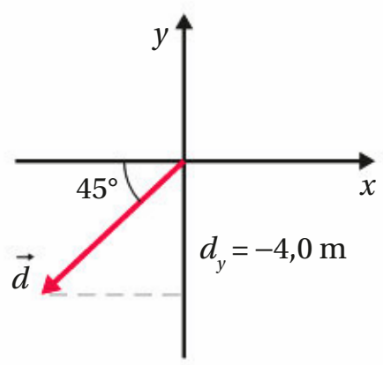
\includegraphics[scale=0.35]{vettored.png}   \end{center} \end{figure}\\
{$A$}: 5,7 m; -4,0 m\ \ {$B$}: 5,7 m; 4,0 m\ \ {$C$}: -5,7 m; 4,0 m\ \ {$D$}: -5,7 m; -4,0 m\ \ 

\mcquestionfooter



\def\mcquestionnumber{9}


\mcquestionheader Seguendo la mappa di un tesoro, un pirata cammina per 2,00~km verso nord-est, poi per 5,00~km verso est, quindi per 2,00~km verso sud-est e infine per 3,00~km verso ovest. Arrivato alla fine del percorso a che distanza si trova dalla posizione che occupava alla partenza?\\
{$A$}: 6,32 km\ \ {$B$}: 4,76 km\ \ {$C$}: 4,59 km\ \ {$D$}: 4,83 km\ \ 

\mcquestionfooter



\def\mcquestionnumber{10}


\mcquestionheader In quale anno il COVID ha fatto la sua comparsa?\\
{$A$}: 2019\ \ {$B$}: 1943\ \ {$C$}: 2020\ \ {$D$}: 2001\ \ 

\mcquestionfooter



\def\mcquestionnumber{11}


\mcquestionheader I due vettori $\vec{a}$ e $\vec{b}$ hanno lo stesso modulo e la stessa direzione. Quale delle seguenti affermazioni è falsa?\\
{$A$}: La loro somma non può mai essere zero\ \ {$B$}: I due vettori sono sicuramente uguali\ \ {$C$}: Tutte le altre\ \ {$D$}: La loro somma è sicuramente nulla\ \ 

\mcquestionfooter



\def\mcquestionnumber{12}


\mcquestionheader Di che colore era il cavallo bianco di Napoleone?\\
{$A$}: Verde\ \ {$B$}: Marrone\ \ {$C$}: Bianco\ \ {$D$}: Blu\ \ 

\mcquestionfooter



\mcpaperfooter

\def\mcserialnumber{14}
\mcpaperheader


\def\mcquestionnumber{1}


\mcquestionheader Qual è la capitale d’Italia?\\
{$A$}: Parigi\ \ {$B$}: Milano\ \ {$C$}: Berlino\ \ {$D$}: Roma\ \ 

\mcquestionfooter



\def\mcquestionnumber{2}


\mcquestionheader Raddoppiando la distanza tra due cariche elettriche puntiformi, la forza elettrostatica diminuisce del\\
{$A$}: 75\%\ \ {$B$}: 90\%\ \ {$C$}: 25\%\ \ {$D$}: 50\%\ \ 

\mcquestionfooter



\def\mcquestionnumber{3}


\mcquestionheader Seguendo la mappa di un tesoro, un pirata cammina per 2,00~km verso nord-est, poi per 5,00~km verso est, quindi per 2,00~km verso sud-est e infine per 3,00~km verso ovest. Arrivato alla fine del percorso a che distanza si trova dalla posizione che occupava alla partenza?\\
{$A$}: 4,83 km\ \ {$B$}: 4,76 km\ \ {$C$}: 4,59 km\ \ {$D$}: 6,32 km\ \ 

\mcquestionfooter



\def\mcquestionnumber{4}


\mcquestionheader Un gatto percorre 90,0~m verso sud e poi prosegue per altri 120~m verso ovest. Lo spostamento e la distanza percorsa sono rispettivamente\\
{$A$}: 210~m e 210~m\ \ {$B$}: 30~m e 210~m\ \ {$C$}: 150~m e 210~m\ \ {$D$}: 210~m e 150~m\ \ 

\mcquestionfooter



\def\mcquestionnumber{5}


\mcquestionheader Il modulo del vettore $\vec{A}(3;4)$ è\\
{$A$}: 5\ \ {$B$}: 8\ \ {$C$}: 12\ \ 

\mcquestionfooter



\def\mcquestionnumber{6}


\mcquestionheader In quale anno il COVID ha fatto la sua comparsa?\\
{$A$}: 2019\ \ {$B$}: 2020\ \ {$C$}: 1943\ \ {$D$}: 2001\ \ 

\mcquestionfooter



\def\mcquestionnumber{7}


\mcquestionheader In che anno pare sia nato Gesù?\\
{$A$}: -80\ \ {$B$}: 0\ \ {$C$}: 20\ \ {$D$}: 2019\ \ 

\mcquestionfooter



\def\mcquestionnumber{8}


\mcquestionheader Dato il vettore $\vec{d}$ in figura, determina il modulo e la componente $d_x$: \begin{figure}[h!]   \begin{center}     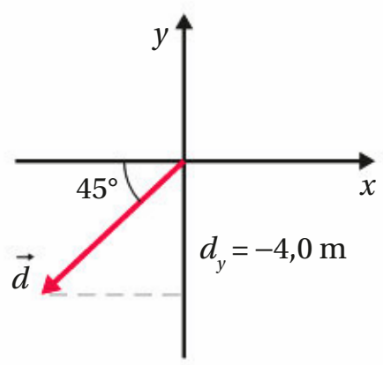
\includegraphics[scale=0.35]{vettored.png}   \end{center} \end{figure}\\
{$A$}: 5,7 m; -4,0 m\ \ {$B$}: -5,7 m; -4,0 m\ \ {$C$}: -5,7 m; 4,0 m\ \ {$D$}: 5,7 m; 4,0 m\ \ 

\mcquestionfooter



\def\mcquestionnumber{9}


\mcquestionheader I due vettori $\vec{a}$ e $\vec{b}$ hanno lo stesso modulo e la stessa direzione. Quale delle seguenti affermazioni è falsa?\\
{$A$}: Tutte le altre\ \ {$B$}: I due vettori sono sicuramente uguali\ \ {$C$}: La loro somma è sicuramente nulla\ \ {$D$}: La loro somma non può mai essere zero\ \ 

\mcquestionfooter



\def\mcquestionnumber{10}


\mcquestionheader Se mischio blu e giallo che colore ottengo?\\
{$A$}: Rosso\ \ {$B$}: Blallo\ \ {$C$}: Verde\ \ {$D$}: Giallu\ \ 

\mcquestionfooter



\def\mcquestionnumber{11}


\mcquestionheader Come si chiama il satellite naturale della Terra?\\
{$A$}: Marte\ \ {$B$}: Sole\ \ {$C$}: ISS\ \ {$D$}: Luna\ \ 

\mcquestionfooter



\def\mcquestionnumber{12}


\mcquestionheader Di che colore era il cavallo bianco di Napoleone?\\
{$A$}: Verde\ \ {$B$}: Bianco\ \ {$C$}: Marrone\ \ {$D$}: Blu\ \ 

\mcquestionfooter



\mcpaperfooter

\def\mcserialnumber{15}
\mcpaperheader


\def\mcquestionnumber{1}


\mcquestionheader Un gatto percorre 90,0~m verso sud e poi prosegue per altri 120~m verso ovest. Lo spostamento e la distanza percorsa sono rispettivamente\\
{$A$}: 150~m e 210~m\ \ {$B$}: 210~m e 210~m\ \ {$C$}: 30~m e 210~m\ \ {$D$}: 210~m e 150~m\ \ 

\mcquestionfooter



\def\mcquestionnumber{2}


\mcquestionheader Come si chiama il satellite naturale della Terra?\\
{$A$}: Luna\ \ {$B$}: Sole\ \ {$C$}: Marte\ \ {$D$}: ISS\ \ 

\mcquestionfooter



\def\mcquestionnumber{3}


\mcquestionheader Se mischio blu e giallo che colore ottengo?\\
{$A$}: Giallu\ \ {$B$}: Rosso\ \ {$C$}: Blallo\ \ {$D$}: Verde\ \ 

\mcquestionfooter



\def\mcquestionnumber{4}


\mcquestionheader Seguendo la mappa di un tesoro, un pirata cammina per 2,00~km verso nord-est, poi per 5,00~km verso est, quindi per 2,00~km verso sud-est e infine per 3,00~km verso ovest. Arrivato alla fine del percorso a che distanza si trova dalla posizione che occupava alla partenza?\\
{$A$}: 4,59 km\ \ {$B$}: 4,76 km\ \ {$C$}: 4,83 km\ \ {$D$}: 6,32 km\ \ 

\mcquestionfooter



\def\mcquestionnumber{5}


\mcquestionheader In che anno pare sia nato Gesù?\\
{$A$}: 0\ \ {$B$}: 20\ \ {$C$}: 2019\ \ {$D$}: -80\ \ 

\mcquestionfooter



\def\mcquestionnumber{6}


\mcquestionheader In quale anno il COVID ha fatto la sua comparsa?\\
{$A$}: 1943\ \ {$B$}: 2019\ \ {$C$}: 2001\ \ {$D$}: 2020\ \ 

\mcquestionfooter



\def\mcquestionnumber{7}


\mcquestionheader Dato il vettore $\vec{d}$ in figura, determina il modulo e la componente $d_x$: \begin{figure}[h!]   \begin{center}     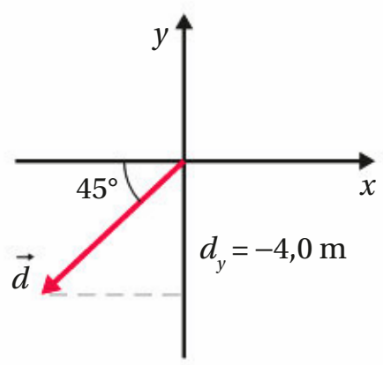
\includegraphics[scale=0.35]{vettored.png}   \end{center} \end{figure}\\
{$A$}: 5,7 m; 4,0 m\ \ {$B$}: -5,7 m; -4,0 m\ \ {$C$}: 5,7 m; -4,0 m\ \ {$D$}: -5,7 m; 4,0 m\ \ 

\mcquestionfooter



\def\mcquestionnumber{8}


\mcquestionheader Qual è la capitale d’Italia?\\
{$A$}: Roma\ \ {$B$}: Berlino\ \ {$C$}: Parigi\ \ {$D$}: Milano\ \ 

\mcquestionfooter



\def\mcquestionnumber{9}


\mcquestionheader Di che colore era il cavallo bianco di Napoleone?\\
{$A$}: Bianco\ \ {$B$}: Marrone\ \ {$C$}: Blu\ \ {$D$}: Verde\ \ 

\mcquestionfooter



\def\mcquestionnumber{10}


\mcquestionheader Il modulo del vettore $\vec{A}(3;4)$ è\\
{$A$}: 12\ \ {$B$}: 8\ \ {$C$}: 5\ \ 

\mcquestionfooter



\def\mcquestionnumber{11}


\mcquestionheader Raddoppiando la distanza tra due cariche elettriche puntiformi, la forza elettrostatica diminuisce del\\
{$A$}: 90\%\ \ {$B$}: 75\%\ \ {$C$}: 50\%\ \ {$D$}: 25\%\ \ 

\mcquestionfooter



\def\mcquestionnumber{12}


\mcquestionheader I due vettori $\vec{a}$ e $\vec{b}$ hanno lo stesso modulo e la stessa direzione. Quale delle seguenti affermazioni è falsa?\\
{$A$}: I due vettori sono sicuramente uguali\ \ {$B$}: La loro somma non può mai essere zero\ \ {$C$}: La loro somma è sicuramente nulla\ \ {$D$}: Tutte le altre\ \ 

\mcquestionfooter



\mcpaperfooter

\def\mcserialnumber{16}
\mcpaperheader


\def\mcquestionnumber{1}


\mcquestionheader Di che colore era il cavallo bianco di Napoleone?\\
{$A$}: Blu\ \ {$B$}: Verde\ \ {$C$}: Marrone\ \ {$D$}: Bianco\ \ 

\mcquestionfooter



\def\mcquestionnumber{2}


\mcquestionheader Come si chiama il satellite naturale della Terra?\\
{$A$}: Marte\ \ {$B$}: Sole\ \ {$C$}: ISS\ \ {$D$}: Luna\ \ 

\mcquestionfooter



\def\mcquestionnumber{3}


\mcquestionheader Seguendo la mappa di un tesoro, un pirata cammina per 2,00~km verso nord-est, poi per 5,00~km verso est, quindi per 2,00~km verso sud-est e infine per 3,00~km verso ovest. Arrivato alla fine del percorso a che distanza si trova dalla posizione che occupava alla partenza?\\
{$A$}: 4,59 km\ \ {$B$}: 6,32 km\ \ {$C$}: 4,83 km\ \ {$D$}: 4,76 km\ \ 

\mcquestionfooter



\def\mcquestionnumber{4}


\mcquestionheader Dato il vettore $\vec{d}$ in figura, determina il modulo e la componente $d_x$: \begin{figure}[h!]   \begin{center}     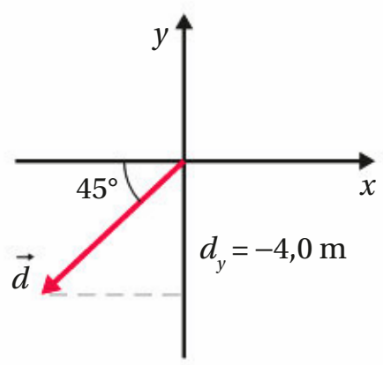
\includegraphics[scale=0.35]{vettored.png}   \end{center} \end{figure}\\
{$A$}: 5,7 m; -4,0 m\ \ {$B$}: 5,7 m; 4,0 m\ \ {$C$}: -5,7 m; 4,0 m\ \ {$D$}: -5,7 m; -4,0 m\ \ 

\mcquestionfooter



\def\mcquestionnumber{5}


\mcquestionheader In quale anno il COVID ha fatto la sua comparsa?\\
{$A$}: 2019\ \ {$B$}: 2001\ \ {$C$}: 1943\ \ {$D$}: 2020\ \ 

\mcquestionfooter



\def\mcquestionnumber{6}


\mcquestionheader Un gatto percorre 90,0~m verso sud e poi prosegue per altri 120~m verso ovest. Lo spostamento e la distanza percorsa sono rispettivamente\\
{$A$}: 210~m e 150~m\ \ {$B$}: 150~m e 210~m\ \ {$C$}: 30~m e 210~m\ \ {$D$}: 210~m e 210~m\ \ 

\mcquestionfooter



\def\mcquestionnumber{7}


\mcquestionheader In che anno pare sia nato Gesù?\\
{$A$}: -80\ \ {$B$}: 2019\ \ {$C$}: 20\ \ {$D$}: 0\ \ 

\mcquestionfooter



\def\mcquestionnumber{8}


\mcquestionheader Il modulo del vettore $\vec{A}(3;4)$ è\\
{$A$}: 5\ \ {$B$}: 8\ \ {$C$}: 12\ \ 

\mcquestionfooter



\def\mcquestionnumber{9}


\mcquestionheader I due vettori $\vec{a}$ e $\vec{b}$ hanno lo stesso modulo e la stessa direzione. Quale delle seguenti affermazioni è falsa?\\
{$A$}: Tutte le altre\ \ {$B$}: La loro somma è sicuramente nulla\ \ {$C$}: I due vettori sono sicuramente uguali\ \ {$D$}: La loro somma non può mai essere zero\ \ 

\mcquestionfooter



\def\mcquestionnumber{10}


\mcquestionheader Se mischio blu e giallo che colore ottengo?\\
{$A$}: Giallu\ \ {$B$}: Blallo\ \ {$C$}: Rosso\ \ {$D$}: Verde\ \ 

\mcquestionfooter



\def\mcquestionnumber{11}


\mcquestionheader Qual è la capitale d’Italia?\\
{$A$}: Roma\ \ {$B$}: Parigi\ \ {$C$}: Berlino\ \ {$D$}: Milano\ \ 

\mcquestionfooter



\def\mcquestionnumber{12}


\mcquestionheader Raddoppiando la distanza tra due cariche elettriche puntiformi, la forza elettrostatica diminuisce del\\
{$A$}: 50\%\ \ {$B$}: 25\%\ \ {$C$}: 75\%\ \ {$D$}: 90\%\ \ 

\mcquestionfooter



\mcpaperfooter

\def\mcserialnumber{17}
\mcpaperheader


\def\mcquestionnumber{1}


\mcquestionheader Come si chiama il satellite naturale della Terra?\\
{$A$}: Sole\ \ {$B$}: Marte\ \ {$C$}: ISS\ \ {$D$}: Luna\ \ 

\mcquestionfooter



\def\mcquestionnumber{2}


\mcquestionheader I due vettori $\vec{a}$ e $\vec{b}$ hanno lo stesso modulo e la stessa direzione. Quale delle seguenti affermazioni è falsa?\\
{$A$}: La loro somma non può mai essere zero\ \ {$B$}: I due vettori sono sicuramente uguali\ \ {$C$}: La loro somma è sicuramente nulla\ \ {$D$}: Tutte le altre\ \ 

\mcquestionfooter



\def\mcquestionnumber{3}


\mcquestionheader In che anno pare sia nato Gesù?\\
{$A$}: -80\ \ {$B$}: 2019\ \ {$C$}: 0\ \ {$D$}: 20\ \ 

\mcquestionfooter



\def\mcquestionnumber{4}


\mcquestionheader Seguendo la mappa di un tesoro, un pirata cammina per 2,00~km verso nord-est, poi per 5,00~km verso est, quindi per 2,00~km verso sud-est e infine per 3,00~km verso ovest. Arrivato alla fine del percorso a che distanza si trova dalla posizione che occupava alla partenza?\\
{$A$}: 4,59 km\ \ {$B$}: 4,83 km\ \ {$C$}: 6,32 km\ \ {$D$}: 4,76 km\ \ 

\mcquestionfooter



\def\mcquestionnumber{5}


\mcquestionheader Di che colore era il cavallo bianco di Napoleone?\\
{$A$}: Bianco\ \ {$B$}: Verde\ \ {$C$}: Marrone\ \ {$D$}: Blu\ \ 

\mcquestionfooter



\def\mcquestionnumber{6}


\mcquestionheader Un gatto percorre 90,0~m verso sud e poi prosegue per altri 120~m verso ovest. Lo spostamento e la distanza percorsa sono rispettivamente\\
{$A$}: 150~m e 210~m\ \ {$B$}: 210~m e 150~m\ \ {$C$}: 30~m e 210~m\ \ {$D$}: 210~m e 210~m\ \ 

\mcquestionfooter



\def\mcquestionnumber{7}


\mcquestionheader Il modulo del vettore $\vec{A}(2;2)$ è\\
{$A$}: boh\ \ {$B$}: chissà\ \ {$C$}: non so\ \ 

\mcquestionfooter



\def\mcquestionnumber{8}


\mcquestionheader Dato il vettore $\vec{d}$ in figura, determina il modulo e la componente $d_x$: \begin{figure}[h!]   \begin{center}     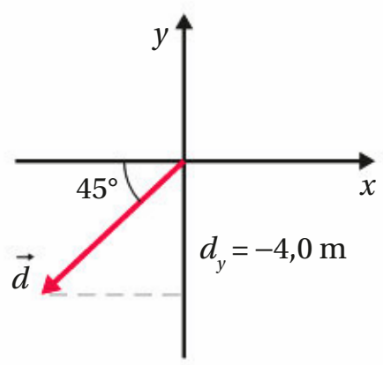
\includegraphics[scale=0.35]{vettored.png}   \end{center} \end{figure}\\
{$A$}: 5,7 m; -4,0 m\ \ {$B$}: -5,7 m; 4,0 m\ \ {$C$}: -5,7 m; -4,0 m\ \ {$D$}: 5,7 m; 4,0 m\ \ 

\mcquestionfooter



\def\mcquestionnumber{9}


\mcquestionheader Qual è la capitale d’Italia?\\
{$A$}: Milano\ \ {$B$}: Roma\ \ {$C$}: Berlino\ \ {$D$}: Parigi\ \ 

\mcquestionfooter



\def\mcquestionnumber{10}


\mcquestionheader Raddoppiando la distanza tra due cariche elettriche puntiformi, la forza elettrostatica diminuisce del\\
{$A$}: 90\%\ \ {$B$}: 75\%\ \ {$C$}: 50\%\ \ {$D$}: 25\%\ \ 

\mcquestionfooter



\def\mcquestionnumber{11}


\mcquestionheader In quale anno il COVID ha fatto la sua comparsa?\\
{$A$}: 2019\ \ {$B$}: 2020\ \ {$C$}: 2001\ \ {$D$}: 1943\ \ 

\mcquestionfooter



\def\mcquestionnumber{12}


\mcquestionheader Se mischio blu e giallo che colore ottengo?\\
{$A$}: Giallu\ \ {$B$}: Verde\ \ {$C$}: Blallo\ \ {$D$}: Rosso\ \ 

\mcquestionfooter



\mcpaperfooter

\def\mcserialnumber{18}
\mcpaperheader


\def\mcquestionnumber{1}


\mcquestionheader In che anno pare sia nato Gesù?\\
{$A$}: 2019\ \ {$B$}: -80\ \ {$C$}: 0\ \ {$D$}: 20\ \ 

\mcquestionfooter



\def\mcquestionnumber{2}


\mcquestionheader Qual è la capitale d’Italia?\\
{$A$}: Berlino\ \ {$B$}: Roma\ \ {$C$}: Milano\ \ {$D$}: Parigi\ \ 

\mcquestionfooter



\def\mcquestionnumber{3}


\mcquestionheader Il modulo del vettore $\vec{A}(2;2)$ è\\
{$A$}: boh\ \ {$B$}: chissà\ \ {$C$}: non so\ \ 

\mcquestionfooter



\def\mcquestionnumber{4}


\mcquestionheader Seguendo la mappa di un tesoro, un pirata cammina per 2,00~km verso nord-est, poi per 5,00~km verso est, quindi per 2,00~km verso sud-est e infine per 3,00~km verso ovest. Arrivato alla fine del percorso a che distanza si trova dalla posizione che occupava alla partenza?\\
{$A$}: 6,32 km\ \ {$B$}: 4,59 km\ \ {$C$}: 4,76 km\ \ {$D$}: 4,83 km\ \ 

\mcquestionfooter



\def\mcquestionnumber{5}


\mcquestionheader Di che colore era il cavallo bianco di Napoleone?\\
{$A$}: Verde\ \ {$B$}: Marrone\ \ {$C$}: Blu\ \ {$D$}: Bianco\ \ 

\mcquestionfooter



\def\mcquestionnumber{6}


\mcquestionheader Se mischio blu e giallo che colore ottengo?\\
{$A$}: Blallo\ \ {$B$}: Giallu\ \ {$C$}: Verde\ \ {$D$}: Rosso\ \ 

\mcquestionfooter



\def\mcquestionnumber{7}


\mcquestionheader In quale anno il COVID ha fatto la sua comparsa?\\
{$A$}: 1943\ \ {$B$}: 2001\ \ {$C$}: 2019\ \ {$D$}: 2020\ \ 

\mcquestionfooter



\def\mcquestionnumber{8}


\mcquestionheader Raddoppiando la distanza tra due cariche elettriche puntiformi, la forza elettrostatica diminuisce del\\
{$A$}: 25\%\ \ {$B$}: 50\%\ \ {$C$}: 75\%\ \ {$D$}: 90\%\ \ 

\mcquestionfooter



\def\mcquestionnumber{9}


\mcquestionheader Come si chiama il satellite naturale della Terra?\\
{$A$}: ISS\ \ {$B$}: Marte\ \ {$C$}: Luna\ \ {$D$}: Sole\ \ 

\mcquestionfooter



\def\mcquestionnumber{10}


\mcquestionheader Dato il vettore $\vec{d}$ in figura, determina il modulo e la componente $d_x$: \begin{figure}[h!]   \begin{center}     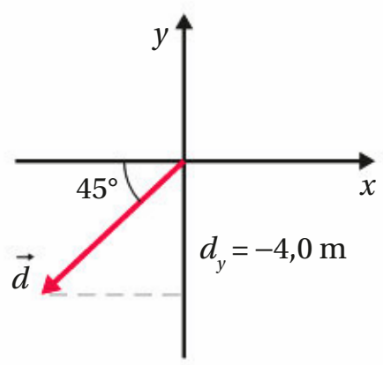
\includegraphics[scale=0.35]{vettored.png}   \end{center} \end{figure}\\
{$A$}: 5,7 m; -4,0 m\ \ {$B$}: 5,7 m; 4,0 m\ \ {$C$}: -5,7 m; -4,0 m\ \ {$D$}: -5,7 m; 4,0 m\ \ 

\mcquestionfooter



\def\mcquestionnumber{11}


\mcquestionheader Un gatto percorre 90,0~m verso sud e poi prosegue per altri 120~m verso ovest. Lo spostamento e la distanza percorsa sono rispettivamente\\
{$A$}: 210~m e 210~m\ \ {$B$}: 150~m e 210~m\ \ {$C$}: 210~m e 150~m\ \ {$D$}: 30~m e 210~m\ \ 

\mcquestionfooter



\def\mcquestionnumber{12}


\mcquestionheader I due vettori $\vec{a}$ e $\vec{b}$ hanno lo stesso modulo e la stessa direzione. Quale delle seguenti affermazioni è falsa?\\
{$A$}: Tutte le altre\ \ {$B$}: La loro somma non può mai essere zero\ \ {$C$}: La loro somma è sicuramente nulla\ \ {$D$}: I due vettori sono sicuramente uguali\ \ 

\mcquestionfooter



\mcpaperfooter

\def\mcserialnumber{19}
\mcpaperheader


\def\mcquestionnumber{1}


\mcquestionheader In che anno pare sia nato Gesù?\\
{$A$}: 2019\ \ {$B$}: 0\ \ {$C$}: 20\ \ {$D$}: -80\ \ 

\mcquestionfooter



\def\mcquestionnumber{2}


\mcquestionheader Il modulo del vettore $\vec{A}(2;2)$ è\\
{$A$}: boh\ \ {$B$}: non so\ \ {$C$}: chissà\ \ 

\mcquestionfooter



\def\mcquestionnumber{3}


\mcquestionheader I due vettori $\vec{a}$ e $\vec{b}$ hanno lo stesso modulo e la stessa direzione. Quale delle seguenti affermazioni è falsa?\\
{$A$}: La loro somma non può mai essere zero\ \ {$B$}: Tutte le altre\ \ {$C$}: La loro somma è sicuramente nulla\ \ {$D$}: I due vettori sono sicuramente uguali\ \ 

\mcquestionfooter



\def\mcquestionnumber{4}


\mcquestionheader In quale anno il COVID ha fatto la sua comparsa?\\
{$A$}: 1943\ \ {$B$}: 2001\ \ {$C$}: 2020\ \ {$D$}: 2019\ \ 

\mcquestionfooter



\def\mcquestionnumber{5}


\mcquestionheader Qual è la capitale d’Italia?\\
{$A$}: Milano\ \ {$B$}: Parigi\ \ {$C$}: Roma\ \ {$D$}: Berlino\ \ 

\mcquestionfooter



\def\mcquestionnumber{6}


\mcquestionheader Di che colore era il cavallo bianco di Napoleone?\\
{$A$}: Marrone\ \ {$B$}: Verde\ \ {$C$}: Blu\ \ {$D$}: Bianco\ \ 

\mcquestionfooter



\def\mcquestionnumber{7}


\mcquestionheader Dato il vettore $\vec{d}$ in figura, determina il modulo e la componente $d_x$: \begin{figure}[h!]   \begin{center}     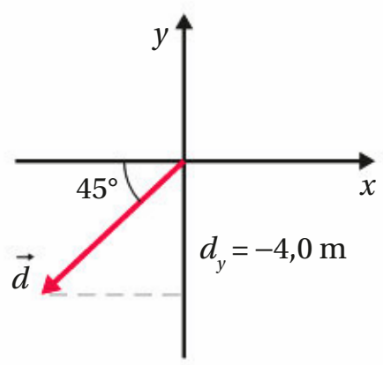
\includegraphics[scale=0.35]{vettored.png}   \end{center} \end{figure}\\
{$A$}: -5,7 m; 4,0 m\ \ {$B$}: 5,7 m; 4,0 m\ \ {$C$}: -5,7 m; -4,0 m\ \ {$D$}: 5,7 m; -4,0 m\ \ 

\mcquestionfooter



\def\mcquestionnumber{8}


\mcquestionheader Un gatto percorre 90,0~m verso sud e poi prosegue per altri 120~m verso ovest. Lo spostamento e la distanza percorsa sono rispettivamente\\
{$A$}: 210~m e 210~m\ \ {$B$}: 150~m e 210~m\ \ {$C$}: 210~m e 150~m\ \ {$D$}: 30~m e 210~m\ \ 

\mcquestionfooter



\def\mcquestionnumber{9}


\mcquestionheader Se mischio blu e giallo che colore ottengo?\\
{$A$}: Verde\ \ {$B$}: Blallo\ \ {$C$}: Giallu\ \ {$D$}: Rosso\ \ 

\mcquestionfooter



\def\mcquestionnumber{10}


\mcquestionheader Seguendo la mappa di un tesoro, un pirata cammina per 2,00~km verso nord-est, poi per 5,00~km verso est, quindi per 2,00~km verso sud-est e infine per 3,00~km verso ovest. Arrivato alla fine del percorso a che distanza si trova dalla posizione che occupava alla partenza?\\
{$A$}: 6,32 km\ \ {$B$}: 4,59 km\ \ {$C$}: 4,83 km\ \ {$D$}: 4,76 km\ \ 

\mcquestionfooter



\def\mcquestionnumber{11}


\mcquestionheader Raddoppiando la distanza tra due cariche elettriche puntiformi, la forza elettrostatica diminuisce del\\
{$A$}: 90\%\ \ {$B$}: 50\%\ \ {$C$}: 25\%\ \ {$D$}: 75\%\ \ 

\mcquestionfooter



\def\mcquestionnumber{12}


\mcquestionheader Come si chiama il satellite naturale della Terra?\\
{$A$}: Luna\ \ {$B$}: Sole\ \ {$C$}: ISS\ \ {$D$}: Marte\ \ 

\mcquestionfooter



\mcpaperfooter

\def\mcserialnumber{20}
\mcpaperheader


\def\mcquestionnumber{1}


\mcquestionheader Seguendo la mappa di un tesoro, un pirata cammina per 2,00~km verso nord-est, poi per 5,00~km verso est, quindi per 2,00~km verso sud-est e infine per 3,00~km verso ovest. Arrivato alla fine del percorso a che distanza si trova dalla posizione che occupava alla partenza?\\
{$A$}: 6,32 km\ \ {$B$}: 4,59 km\ \ {$C$}: 4,76 km\ \ {$D$}: 4,83 km\ \ 

\mcquestionfooter



\def\mcquestionnumber{2}


\mcquestionheader In quale anno il COVID ha fatto la sua comparsa?\\
{$A$}: 2019\ \ {$B$}: 2020\ \ {$C$}: 1943\ \ {$D$}: 2001\ \ 

\mcquestionfooter



\def\mcquestionnumber{3}


\mcquestionheader Di che colore era il cavallo bianco di Napoleone?\\
{$A$}: Marrone\ \ {$B$}: Blu\ \ {$C$}: Verde\ \ {$D$}: Bianco\ \ 

\mcquestionfooter



\def\mcquestionnumber{4}


\mcquestionheader I due vettori $\vec{a}$ e $\vec{b}$ hanno lo stesso modulo e la stessa direzione. Quale delle seguenti affermazioni è falsa?\\
{$A$}: La loro somma è sicuramente nulla\ \ {$B$}: I due vettori sono sicuramente uguali\ \ {$C$}: La loro somma non può mai essere zero\ \ {$D$}: Tutte le altre\ \ 

\mcquestionfooter



\def\mcquestionnumber{5}


\mcquestionheader Qual è la capitale d’Italia?\\
{$A$}: Roma\ \ {$B$}: Parigi\ \ {$C$}: Milano\ \ {$D$}: Berlino\ \ 

\mcquestionfooter



\def\mcquestionnumber{6}


\mcquestionheader In che anno pare sia nato Gesù?\\
{$A$}: 20\ \ {$B$}: 0\ \ {$C$}: -80\ \ {$D$}: 2019\ \ 

\mcquestionfooter



\def\mcquestionnumber{7}


\mcquestionheader Un gatto percorre 90,0~m verso sud e poi prosegue per altri 120~m verso ovest. Lo spostamento e la distanza percorsa sono rispettivamente\\
{$A$}: 30~m e 210~m\ \ {$B$}: 210~m e 150~m\ \ {$C$}: 210~m e 210~m\ \ {$D$}: 150~m e 210~m\ \ 

\mcquestionfooter



\def\mcquestionnumber{8}


\mcquestionheader Come si chiama il satellite naturale della Terra?\\
{$A$}: Marte\ \ {$B$}: ISS\ \ {$C$}: Luna\ \ {$D$}: Sole\ \ 

\mcquestionfooter



\def\mcquestionnumber{9}


\mcquestionheader Il modulo del vettore $\vec{A}(2;2)$ è\\
{$A$}: non so\ \ {$B$}: boh\ \ {$C$}: chissà\ \ 

\mcquestionfooter



\def\mcquestionnumber{10}


\mcquestionheader Raddoppiando la distanza tra due cariche elettriche puntiformi, la forza elettrostatica diminuisce del\\
{$A$}: 25\%\ \ {$B$}: 75\%\ \ {$C$}: 90\%\ \ {$D$}: 50\%\ \ 

\mcquestionfooter



\def\mcquestionnumber{11}


\mcquestionheader Se mischio blu e giallo che colore ottengo?\\
{$A$}: Rosso\ \ {$B$}: Giallu\ \ {$C$}: Verde\ \ {$D$}: Blallo\ \ 

\mcquestionfooter



\def\mcquestionnumber{12}


\mcquestionheader Dato il vettore $\vec{d}$ in figura, determina il modulo e la componente $d_x$: \begin{figure}[h!]   \begin{center}     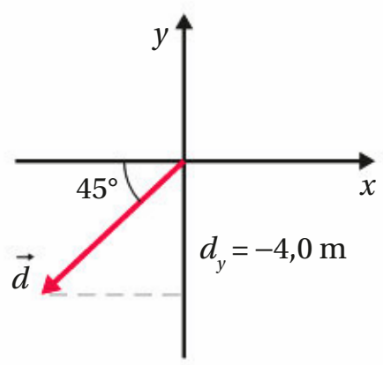
\includegraphics[scale=0.35]{vettored.png}   \end{center} \end{figure}\\
{$A$}: 5,7 m; -4,0 m\ \ {$B$}: -5,7 m; 4,0 m\ \ {$C$}: -5,7 m; -4,0 m\ \ {$D$}: 5,7 m; 4,0 m\ \ 

\mcquestionfooter



\mcpaperfooter

\def\mcserialnumber{21}
\mcpaperheader


\def\mcquestionnumber{1}


\mcquestionheader Se mischio blu e giallo che colore ottengo?\\
{$A$}: Rosso\ \ {$B$}: Giallu\ \ {$C$}: Verde\ \ {$D$}: Blallo\ \ 

\mcquestionfooter



\def\mcquestionnumber{2}


\mcquestionheader Raddoppiando la distanza tra due cariche elettriche puntiformi, la forza elettrostatica diminuisce del\\
{$A$}: 50\%\ \ {$B$}: 75\%\ \ {$C$}: 25\%\ \ {$D$}: 90\%\ \ 

\mcquestionfooter



\def\mcquestionnumber{3}


\mcquestionheader In che anno pare sia nato Gesù?\\
{$A$}: 0\ \ {$B$}: 2019\ \ {$C$}: 20\ \ {$D$}: -80\ \ 

\mcquestionfooter



\def\mcquestionnumber{4}


\mcquestionheader Qual è la capitale d’Italia?\\
{$A$}: Roma\ \ {$B$}: Parigi\ \ {$C$}: Milano\ \ {$D$}: Berlino\ \ 

\mcquestionfooter



\def\mcquestionnumber{5}


\mcquestionheader In quale anno il COVID ha fatto la sua comparsa?\\
{$A$}: 1943\ \ {$B$}: 2019\ \ {$C$}: 2020\ \ {$D$}: 2001\ \ 

\mcquestionfooter



\def\mcquestionnumber{6}


\mcquestionheader Seguendo la mappa di un tesoro, un pirata cammina per 2,00~km verso nord-est, poi per 5,00~km verso est, quindi per 2,00~km verso sud-est e infine per 3,00~km verso ovest. Arrivato alla fine del percorso a che distanza si trova dalla posizione che occupava alla partenza?\\
{$A$}: 4,76 km\ \ {$B$}: 4,83 km\ \ {$C$}: 4,59 km\ \ {$D$}: 6,32 km\ \ 

\mcquestionfooter



\def\mcquestionnumber{7}


\mcquestionheader Come si chiama il satellite naturale della Terra?\\
{$A$}: Marte\ \ {$B$}: Luna\ \ {$C$}: Sole\ \ {$D$}: ISS\ \ 

\mcquestionfooter



\def\mcquestionnumber{8}


\mcquestionheader Il modulo del vettore $\vec{A}(2;2)$ è\\
{$A$}: non so\ \ {$B$}: boh\ \ {$C$}: chissà\ \ 

\mcquestionfooter



\def\mcquestionnumber{9}


\mcquestionheader Dato il vettore $\vec{d}$ in figura, determina il modulo e la componente $d_x$: \begin{figure}[h!]   \begin{center}     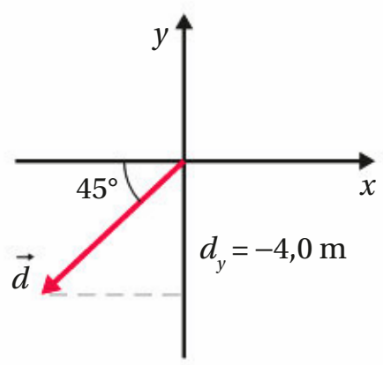
\includegraphics[scale=0.35]{vettored.png}   \end{center} \end{figure}\\
{$A$}: -5,7 m; -4,0 m\ \ {$B$}: 5,7 m; 4,0 m\ \ {$C$}: -5,7 m; 4,0 m\ \ {$D$}: 5,7 m; -4,0 m\ \ 

\mcquestionfooter



\def\mcquestionnumber{10}


\mcquestionheader I due vettori $\vec{a}$ e $\vec{b}$ hanno lo stesso modulo e la stessa direzione. Quale delle seguenti affermazioni è falsa?\\
{$A$}: La loro somma è sicuramente nulla\ \ {$B$}: Tutte le altre\ \ {$C$}: La loro somma non può mai essere zero\ \ {$D$}: I due vettori sono sicuramente uguali\ \ 

\mcquestionfooter



\def\mcquestionnumber{11}


\mcquestionheader Un gatto percorre 90,0~m verso sud e poi prosegue per altri 120~m verso ovest. Lo spostamento e la distanza percorsa sono rispettivamente\\
{$A$}: 210~m e 210~m\ \ {$B$}: 150~m e 210~m\ \ {$C$}: 30~m e 210~m\ \ {$D$}: 210~m e 150~m\ \ 

\mcquestionfooter



\def\mcquestionnumber{12}


\mcquestionheader Di che colore era il cavallo bianco di Napoleone?\\
{$A$}: Verde\ \ {$B$}: Blu\ \ {$C$}: Marrone\ \ {$D$}: Bianco\ \ 

\mcquestionfooter



\mcpaperfooter

\def\mcserialnumber{22}
\mcpaperheader


\def\mcquestionnumber{1}


\mcquestionheader Raddoppiando la distanza tra due cariche elettriche puntiformi, la forza elettrostatica diminuisce del\\
{$A$}: 90\%\ \ {$B$}: 25\%\ \ {$C$}: 75\%\ \ {$D$}: 50\%\ \ 

\mcquestionfooter



\def\mcquestionnumber{2}


\mcquestionheader Seguendo la mappa di un tesoro, un pirata cammina per 2,00~km verso nord-est, poi per 5,00~km verso est, quindi per 2,00~km verso sud-est e infine per 3,00~km verso ovest. Arrivato alla fine del percorso a che distanza si trova dalla posizione che occupava alla partenza?\\
{$A$}: 6,32 km\ \ {$B$}: 4,59 km\ \ {$C$}: 4,83 km\ \ {$D$}: 4,76 km\ \ 

\mcquestionfooter



\def\mcquestionnumber{3}


\mcquestionheader Come si chiama il satellite naturale della Terra?\\
{$A$}: Sole\ \ {$B$}: Marte\ \ {$C$}: ISS\ \ {$D$}: Luna\ \ 

\mcquestionfooter



\def\mcquestionnumber{4}


\mcquestionheader Il modulo del vettore $\vec{A}(3;4)$ è\\
{$A$}: 8\ \ {$B$}: 12\ \ {$C$}: 5\ \ 

\mcquestionfooter



\def\mcquestionnumber{5}


\mcquestionheader I due vettori $\vec{a}$ e $\vec{b}$ hanno lo stesso modulo e la stessa direzione. Quale delle seguenti affermazioni è falsa?\\
{$A$}: I due vettori sono sicuramente uguali\ \ {$B$}: La loro somma non può mai essere zero\ \ {$C$}: La loro somma è sicuramente nulla\ \ {$D$}: Tutte le altre\ \ 

\mcquestionfooter



\def\mcquestionnumber{6}


\mcquestionheader In che anno pare sia nato Gesù?\\
{$A$}: 20\ \ {$B$}: 0\ \ {$C$}: -80\ \ {$D$}: 2019\ \ 

\mcquestionfooter



\def\mcquestionnumber{7}


\mcquestionheader Dato il vettore $\vec{d}$ in figura, determina il modulo e la componente $d_x$: \begin{figure}[h!]   \begin{center}     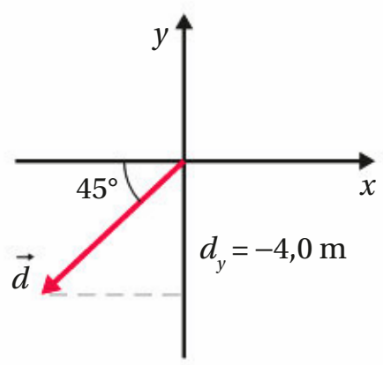
\includegraphics[scale=0.35]{vettored.png}   \end{center} \end{figure}\\
{$A$}: 5,7 m; -4,0 m\ \ {$B$}: -5,7 m; -4,0 m\ \ {$C$}: 5,7 m; 4,0 m\ \ {$D$}: -5,7 m; 4,0 m\ \ 

\mcquestionfooter



\def\mcquestionnumber{8}


\mcquestionheader Un gatto percorre 90,0~m verso sud e poi prosegue per altri 120~m verso ovest. Lo spostamento e la distanza percorsa sono rispettivamente\\
{$A$}: 210~m e 150~m\ \ {$B$}: 210~m e 210~m\ \ {$C$}: 150~m e 210~m\ \ {$D$}: 30~m e 210~m\ \ 

\mcquestionfooter



\def\mcquestionnumber{9}


\mcquestionheader In quale anno il COVID ha fatto la sua comparsa?\\
{$A$}: 2020\ \ {$B$}: 1943\ \ {$C$}: 2001\ \ {$D$}: 2019\ \ 

\mcquestionfooter



\def\mcquestionnumber{10}


\mcquestionheader Se mischio blu e giallo che colore ottengo?\\
{$A$}: Verde\ \ {$B$}: Blallo\ \ {$C$}: Giallu\ \ {$D$}: Rosso\ \ 

\mcquestionfooter



\def\mcquestionnumber{11}


\mcquestionheader Di che colore era il cavallo bianco di Napoleone?\\
{$A$}: Blu\ \ {$B$}: Verde\ \ {$C$}: Marrone\ \ {$D$}: Bianco\ \ 

\mcquestionfooter



\def\mcquestionnumber{12}


\mcquestionheader Qual è la capitale d’Italia?\\
{$A$}: Milano\ \ {$B$}: Parigi\ \ {$C$}: Roma\ \ {$D$}: Berlino\ \ 

\mcquestionfooter



\mcpaperfooter

\def\mcserialnumber{23}
\mcpaperheader


\def\mcquestionnumber{1}


\mcquestionheader Di che colore era il cavallo bianco di Napoleone?\\
{$A$}: Marrone\ \ {$B$}: Bianco\ \ {$C$}: Verde\ \ {$D$}: Blu\ \ 

\mcquestionfooter



\def\mcquestionnumber{2}


\mcquestionheader Qual è la capitale d’Italia?\\
{$A$}: Milano\ \ {$B$}: Roma\ \ {$C$}: Parigi\ \ {$D$}: Berlino\ \ 

\mcquestionfooter



\def\mcquestionnumber{3}


\mcquestionheader Seguendo la mappa di un tesoro, un pirata cammina per 2,00~km verso nord-est, poi per 5,00~km verso est, quindi per 2,00~km verso sud-est e infine per 3,00~km verso ovest. Arrivato alla fine del percorso a che distanza si trova dalla posizione che occupava alla partenza?\\
{$A$}: 4,59 km\ \ {$B$}: 4,76 km\ \ {$C$}: 4,83 km\ \ {$D$}: 6,32 km\ \ 

\mcquestionfooter



\def\mcquestionnumber{4}


\mcquestionheader Come si chiama il satellite naturale della Terra?\\
{$A$}: Marte\ \ {$B$}: Luna\ \ {$C$}: ISS\ \ {$D$}: Sole\ \ 

\mcquestionfooter



\def\mcquestionnumber{5}


\mcquestionheader Raddoppiando la distanza tra due cariche elettriche puntiformi, la forza elettrostatica diminuisce del\\
{$A$}: 75\%\ \ {$B$}: 50\%\ \ {$C$}: 25\%\ \ {$D$}: 90\%\ \ 

\mcquestionfooter



\def\mcquestionnumber{6}


\mcquestionheader In che anno pare sia nato Gesù?\\
{$A$}: 20\ \ {$B$}: 2019\ \ {$C$}: 0\ \ {$D$}: -80\ \ 

\mcquestionfooter



\def\mcquestionnumber{7}


\mcquestionheader Dato il vettore $\vec{d}$ in figura, determina il modulo e la componente $d_x$: \begin{figure}[h!]   \begin{center}     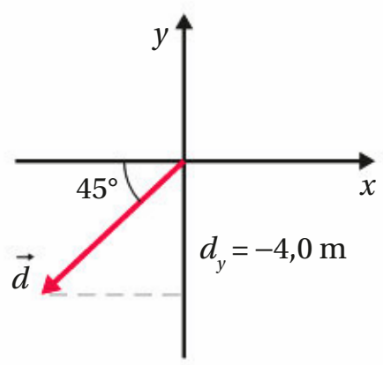
\includegraphics[scale=0.35]{vettored.png}   \end{center} \end{figure}\\
{$A$}: -5,7 m; 4,0 m\ \ {$B$}: -5,7 m; -4,0 m\ \ {$C$}: 5,7 m; -4,0 m\ \ {$D$}: 5,7 m; 4,0 m\ \ 

\mcquestionfooter



\def\mcquestionnumber{8}


\mcquestionheader In quale anno il COVID ha fatto la sua comparsa?\\
{$A$}: 2019\ \ {$B$}: 2020\ \ {$C$}: 2001\ \ {$D$}: 1943\ \ 

\mcquestionfooter



\def\mcquestionnumber{9}


\mcquestionheader Se mischio blu e giallo che colore ottengo?\\
{$A$}: Blallo\ \ {$B$}: Verde\ \ {$C$}: Giallu\ \ {$D$}: Rosso\ \ 

\mcquestionfooter



\def\mcquestionnumber{10}


\mcquestionheader Il modulo del vettore $\vec{A}(3;4)$ è\\
{$A$}: 12\ \ {$B$}: 5\ \ {$C$}: 8\ \ 

\mcquestionfooter



\def\mcquestionnumber{11}


\mcquestionheader I due vettori $\vec{a}$ e $\vec{b}$ hanno lo stesso modulo e la stessa direzione. Quale delle seguenti affermazioni è falsa?\\
{$A$}: La loro somma non può mai essere zero\ \ {$B$}: La loro somma è sicuramente nulla\ \ {$C$}: I due vettori sono sicuramente uguali\ \ {$D$}: Tutte le altre\ \ 

\mcquestionfooter



\def\mcquestionnumber{12}


\mcquestionheader Un gatto percorre 90,0~m verso sud e poi prosegue per altri 120~m verso ovest. Lo spostamento e la distanza percorsa sono rispettivamente\\
{$A$}: 150~m e 210~m\ \ {$B$}: 210~m e 150~m\ \ {$C$}: 210~m e 210~m\ \ {$D$}: 30~m e 210~m\ \ 

\mcquestionfooter



\mcpaperfooter

\def\mcserialnumber{24}
\mcpaperheader


\def\mcquestionnumber{1}


\mcquestionheader Raddoppiando la distanza tra due cariche elettriche puntiformi, la forza elettrostatica diminuisce del\\
{$A$}: 25\%\ \ {$B$}: 90\%\ \ {$C$}: 75\%\ \ {$D$}: 50\%\ \ 

\mcquestionfooter



\def\mcquestionnumber{2}


\mcquestionheader Se mischio blu e giallo che colore ottengo?\\
{$A$}: Verde\ \ {$B$}: Blallo\ \ {$C$}: Giallu\ \ {$D$}: Rosso\ \ 

\mcquestionfooter



\def\mcquestionnumber{3}


\mcquestionheader Qual è la capitale d’Italia?\\
{$A$}: Roma\ \ {$B$}: Milano\ \ {$C$}: Parigi\ \ {$D$}: Berlino\ \ 

\mcquestionfooter



\def\mcquestionnumber{4}


\mcquestionheader In che anno pare sia nato Gesù?\\
{$A$}: 0\ \ {$B$}: 20\ \ {$C$}: -80\ \ {$D$}: 2019\ \ 

\mcquestionfooter



\def\mcquestionnumber{5}


\mcquestionheader Seguendo la mappa di un tesoro, un pirata cammina per 2,00~km verso nord-est, poi per 5,00~km verso est, quindi per 2,00~km verso sud-est e infine per 3,00~km verso ovest. Arrivato alla fine del percorso a che distanza si trova dalla posizione che occupava alla partenza?\\
{$A$}: 4,76 km\ \ {$B$}: 4,83 km\ \ {$C$}: 6,32 km\ \ {$D$}: 4,59 km\ \ 

\mcquestionfooter



\def\mcquestionnumber{6}


\mcquestionheader Il modulo del vettore $\vec{A}(3;4)$ è\\
{$A$}: 8\ \ {$B$}: 5\ \ {$C$}: 12\ \ 

\mcquestionfooter



\def\mcquestionnumber{7}


\mcquestionheader Dato il vettore $\vec{d}$ in figura, determina il modulo e la componente $d_x$: \begin{figure}[h!]   \begin{center}     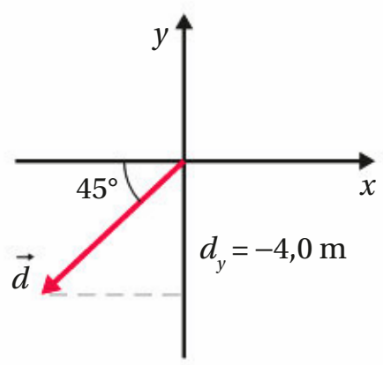
\includegraphics[scale=0.35]{vettored.png}   \end{center} \end{figure}\\
{$A$}: 5,7 m; 4,0 m\ \ {$B$}: 5,7 m; -4,0 m\ \ {$C$}: -5,7 m; 4,0 m\ \ {$D$}: -5,7 m; -4,0 m\ \ 

\mcquestionfooter



\def\mcquestionnumber{8}


\mcquestionheader Come si chiama il satellite naturale della Terra?\\
{$A$}: Sole\ \ {$B$}: Marte\ \ {$C$}: Luna\ \ {$D$}: ISS\ \ 

\mcquestionfooter



\def\mcquestionnumber{9}


\mcquestionheader In quale anno il COVID ha fatto la sua comparsa?\\
{$A$}: 2020\ \ {$B$}: 2001\ \ {$C$}: 1943\ \ {$D$}: 2019\ \ 

\mcquestionfooter



\def\mcquestionnumber{10}


\mcquestionheader Di che colore era il cavallo bianco di Napoleone?\\
{$A$}: Bianco\ \ {$B$}: Marrone\ \ {$C$}: Verde\ \ {$D$}: Blu\ \ 

\mcquestionfooter



\def\mcquestionnumber{11}


\mcquestionheader Un gatto percorre 90,0~m verso sud e poi prosegue per altri 120~m verso ovest. Lo spostamento e la distanza percorsa sono rispettivamente\\
{$A$}: 150~m e 210~m\ \ {$B$}: 210~m e 150~m\ \ {$C$}: 210~m e 210~m\ \ {$D$}: 30~m e 210~m\ \ 

\mcquestionfooter



\def\mcquestionnumber{12}


\mcquestionheader I due vettori $\vec{a}$ e $\vec{b}$ hanno lo stesso modulo e la stessa direzione. Quale delle seguenti affermazioni è falsa?\\
{$A$}: La loro somma è sicuramente nulla\ \ {$B$}: I due vettori sono sicuramente uguali\ \ {$C$}: La loro somma non può mai essere zero\ \ {$D$}: Tutte le altre\ \ 

\mcquestionfooter



\mcpaperfooter

\def\mcserialnumber{25}
\mcpaperheader


\def\mcquestionnumber{1}


\mcquestionheader Seguendo la mappa di un tesoro, un pirata cammina per 2,00~km verso nord-est, poi per 5,00~km verso est, quindi per 2,00~km verso sud-est e infine per 3,00~km verso ovest. Arrivato alla fine del percorso a che distanza si trova dalla posizione che occupava alla partenza?\\
{$A$}: 6,32 km\ \ {$B$}: 4,83 km\ \ {$C$}: 4,59 km\ \ {$D$}: 4,76 km\ \ 

\mcquestionfooter



\def\mcquestionnumber{2}


\mcquestionheader Di che colore era il cavallo bianco di Napoleone?\\
{$A$}: Verde\ \ {$B$}: Bianco\ \ {$C$}: Blu\ \ {$D$}: Marrone\ \ 

\mcquestionfooter



\def\mcquestionnumber{3}


\mcquestionheader Qual è la capitale d’Italia?\\
{$A$}: Berlino\ \ {$B$}: Parigi\ \ {$C$}: Milano\ \ {$D$}: Roma\ \ 

\mcquestionfooter



\def\mcquestionnumber{4}


\mcquestionheader In quale anno il COVID ha fatto la sua comparsa?\\
{$A$}: 1943\ \ {$B$}: 2020\ \ {$C$}: 2019\ \ {$D$}: 2001\ \ 

\mcquestionfooter



\def\mcquestionnumber{5}


\mcquestionheader In che anno pare sia nato Gesù?\\
{$A$}: 20\ \ {$B$}: 0\ \ {$C$}: 2019\ \ {$D$}: -80\ \ 

\mcquestionfooter



\def\mcquestionnumber{6}


\mcquestionheader I due vettori $\vec{a}$ e $\vec{b}$ hanno lo stesso modulo e la stessa direzione. Quale delle seguenti affermazioni è falsa?\\
{$A$}: I due vettori sono sicuramente uguali\ \ {$B$}: Tutte le altre\ \ {$C$}: La loro somma è sicuramente nulla\ \ {$D$}: La loro somma non può mai essere zero\ \ 

\mcquestionfooter



\def\mcquestionnumber{7}


\mcquestionheader Raddoppiando la distanza tra due cariche elettriche puntiformi, la forza elettrostatica diminuisce del\\
{$A$}: 25\%\ \ {$B$}: 75\%\ \ {$C$}: 90\%\ \ {$D$}: 50\%\ \ 

\mcquestionfooter



\def\mcquestionnumber{8}


\mcquestionheader Il modulo del vettore $\vec{A}(2;2)$ è\\
{$A$}: chissà\ \ {$B$}: boh\ \ {$C$}: non so\ \ 

\mcquestionfooter



\def\mcquestionnumber{9}


\mcquestionheader Dato il vettore $\vec{d}$ in figura, determina il modulo e la componente $d_x$: \begin{figure}[h!]   \begin{center}     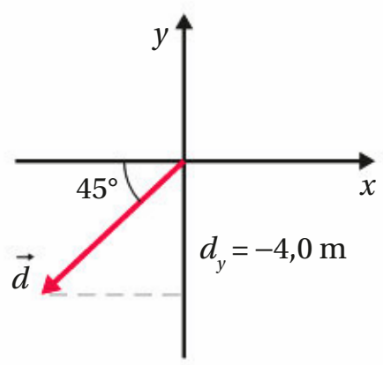
\includegraphics[scale=0.35]{vettored.png}   \end{center} \end{figure}\\
{$A$}: 5,7 m; -4,0 m\ \ {$B$}: -5,7 m; -4,0 m\ \ {$C$}: -5,7 m; 4,0 m\ \ {$D$}: 5,7 m; 4,0 m\ \ 

\mcquestionfooter



\def\mcquestionnumber{10}


\mcquestionheader Se mischio blu e giallo che colore ottengo?\\
{$A$}: Verde\ \ {$B$}: Blallo\ \ {$C$}: Rosso\ \ {$D$}: Giallu\ \ 

\mcquestionfooter



\def\mcquestionnumber{11}


\mcquestionheader Come si chiama il satellite naturale della Terra?\\
{$A$}: Marte\ \ {$B$}: Luna\ \ {$C$}: ISS\ \ {$D$}: Sole\ \ 

\mcquestionfooter



\def\mcquestionnumber{12}


\mcquestionheader Un gatto percorre 90,0~m verso sud e poi prosegue per altri 120~m verso ovest. Lo spostamento e la distanza percorsa sono rispettivamente\\
{$A$}: 30~m e 210~m\ \ {$B$}: 150~m e 210~m\ \ {$C$}: 210~m e 150~m\ \ {$D$}: 210~m e 210~m\ \ 

\mcquestionfooter



\mcpaperfooter

\def\mcserialnumber{26}
\mcpaperheader


\def\mcquestionnumber{1}


\mcquestionheader I due vettori $\vec{a}$ e $\vec{b}$ hanno lo stesso modulo e la stessa direzione. Quale delle seguenti affermazioni è falsa?\\
{$A$}: La loro somma non può mai essere zero\ \ {$B$}: La loro somma è sicuramente nulla\ \ {$C$}: Tutte le altre\ \ {$D$}: I due vettori sono sicuramente uguali\ \ 

\mcquestionfooter



\def\mcquestionnumber{2}


\mcquestionheader Dato il vettore $\vec{d}$ in figura, determina il modulo e la componente $d_x$: \begin{figure}[h!]   \begin{center}     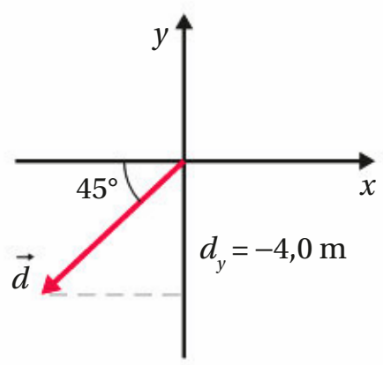
\includegraphics[scale=0.35]{vettored.png}   \end{center} \end{figure}\\
{$A$}: 5,7 m; 4,0 m\ \ {$B$}: -5,7 m; -4,0 m\ \ {$C$}: 5,7 m; -4,0 m\ \ {$D$}: -5,7 m; 4,0 m\ \ 

\mcquestionfooter



\def\mcquestionnumber{3}


\mcquestionheader In quale anno il COVID ha fatto la sua comparsa?\\
{$A$}: 2019\ \ {$B$}: 2020\ \ {$C$}: 1943\ \ {$D$}: 2001\ \ 

\mcquestionfooter



\def\mcquestionnumber{4}


\mcquestionheader Seguendo la mappa di un tesoro, un pirata cammina per 2,00~km verso nord-est, poi per 5,00~km verso est, quindi per 2,00~km verso sud-est e infine per 3,00~km verso ovest. Arrivato alla fine del percorso a che distanza si trova dalla posizione che occupava alla partenza?\\
{$A$}: 6,32 km\ \ {$B$}: 4,59 km\ \ {$C$}: 4,83 km\ \ {$D$}: 4,76 km\ \ 

\mcquestionfooter



\def\mcquestionnumber{5}


\mcquestionheader Raddoppiando la distanza tra due cariche elettriche puntiformi, la forza elettrostatica diminuisce del\\
{$A$}: 75\%\ \ {$B$}: 90\%\ \ {$C$}: 50\%\ \ {$D$}: 25\%\ \ 

\mcquestionfooter



\def\mcquestionnumber{6}


\mcquestionheader Di che colore era il cavallo bianco di Napoleone?\\
{$A$}: Verde\ \ {$B$}: Bianco\ \ {$C$}: Marrone\ \ {$D$}: Blu\ \ 

\mcquestionfooter



\def\mcquestionnumber{7}


\mcquestionheader Come si chiama il satellite naturale della Terra?\\
{$A$}: ISS\ \ {$B$}: Sole\ \ {$C$}: Marte\ \ {$D$}: Luna\ \ 

\mcquestionfooter



\def\mcquestionnumber{8}


\mcquestionheader Un gatto percorre 90,0~m verso sud e poi prosegue per altri 120~m verso ovest. Lo spostamento e la distanza percorsa sono rispettivamente\\
{$A$}: 210~m e 150~m\ \ {$B$}: 210~m e 210~m\ \ {$C$}: 150~m e 210~m\ \ {$D$}: 30~m e 210~m\ \ 

\mcquestionfooter



\def\mcquestionnumber{9}


\mcquestionheader In che anno pare sia nato Gesù?\\
{$A$}: -80\ \ {$B$}: 20\ \ {$C$}: 0\ \ {$D$}: 2019\ \ 

\mcquestionfooter



\def\mcquestionnumber{10}


\mcquestionheader Il modulo del vettore $\vec{A}(3;4)$ è\\
{$A$}: 5\ \ {$B$}: 12\ \ {$C$}: 8\ \ 

\mcquestionfooter



\def\mcquestionnumber{11}


\mcquestionheader Qual è la capitale d’Italia?\\
{$A$}: Berlino\ \ {$B$}: Roma\ \ {$C$}: Milano\ \ {$D$}: Parigi\ \ 

\mcquestionfooter



\def\mcquestionnumber{12}


\mcquestionheader Se mischio blu e giallo che colore ottengo?\\
{$A$}: Giallu\ \ {$B$}: Rosso\ \ {$C$}: Blallo\ \ {$D$}: Verde\ \ 

\mcquestionfooter



\mcpaperfooter

\def\mcserialnumber{27}
\mcpaperheader


\def\mcquestionnumber{1}


\mcquestionheader In quale anno il COVID ha fatto la sua comparsa?\\
{$A$}: 1943\ \ {$B$}: 2001\ \ {$C$}: 2019\ \ {$D$}: 2020\ \ 

\mcquestionfooter



\def\mcquestionnumber{2}


\mcquestionheader Di che colore era il cavallo bianco di Napoleone?\\
{$A$}: Bianco\ \ {$B$}: Verde\ \ {$C$}: Blu\ \ {$D$}: Marrone\ \ 

\mcquestionfooter



\def\mcquestionnumber{3}


\mcquestionheader Dato il vettore $\vec{d}$ in figura, determina il modulo e la componente $d_x$: \begin{figure}[h!]   \begin{center}     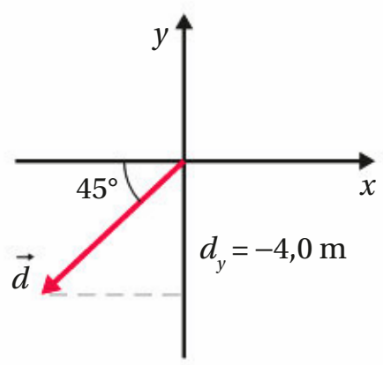
\includegraphics[scale=0.35]{vettored.png}   \end{center} \end{figure}\\
{$A$}: -5,7 m; 4,0 m\ \ {$B$}: -5,7 m; -4,0 m\ \ {$C$}: 5,7 m; 4,0 m\ \ {$D$}: 5,7 m; -4,0 m\ \ 

\mcquestionfooter



\def\mcquestionnumber{4}


\mcquestionheader Qual è la capitale d’Italia?\\
{$A$}: Parigi\ \ {$B$}: Roma\ \ {$C$}: Berlino\ \ {$D$}: Milano\ \ 

\mcquestionfooter



\def\mcquestionnumber{5}


\mcquestionheader Il modulo del vettore $\vec{A}(3;4)$ è\\
{$A$}: 12\ \ {$B$}: 5\ \ {$C$}: 8\ \ 

\mcquestionfooter



\def\mcquestionnumber{6}


\mcquestionheader Come si chiama il satellite naturale della Terra?\\
{$A$}: Luna\ \ {$B$}: Sole\ \ {$C$}: Marte\ \ {$D$}: ISS\ \ 

\mcquestionfooter



\def\mcquestionnumber{7}


\mcquestionheader I due vettori $\vec{a}$ e $\vec{b}$ hanno lo stesso modulo e la stessa direzione. Quale delle seguenti affermazioni è falsa?\\
{$A$}: I due vettori sono sicuramente uguali\ \ {$B$}: Tutte le altre\ \ {$C$}: La loro somma è sicuramente nulla\ \ {$D$}: La loro somma non può mai essere zero\ \ 

\mcquestionfooter



\def\mcquestionnumber{8}


\mcquestionheader Raddoppiando la distanza tra due cariche elettriche puntiformi, la forza elettrostatica diminuisce del\\
{$A$}: 50\%\ \ {$B$}: 25\%\ \ {$C$}: 75\%\ \ {$D$}: 90\%\ \ 

\mcquestionfooter



\def\mcquestionnumber{9}


\mcquestionheader In che anno pare sia nato Gesù?\\
{$A$}: 0\ \ {$B$}: -80\ \ {$C$}: 2019\ \ {$D$}: 20\ \ 

\mcquestionfooter



\def\mcquestionnumber{10}


\mcquestionheader Un gatto percorre 90,0~m verso sud e poi prosegue per altri 120~m verso ovest. Lo spostamento e la distanza percorsa sono rispettivamente\\
{$A$}: 150~m e 210~m\ \ {$B$}: 210~m e 210~m\ \ {$C$}: 210~m e 150~m\ \ {$D$}: 30~m e 210~m\ \ 

\mcquestionfooter



\def\mcquestionnumber{11}


\mcquestionheader Se mischio blu e giallo che colore ottengo?\\
{$A$}: Rosso\ \ {$B$}: Giallu\ \ {$C$}: Verde\ \ {$D$}: Blallo\ \ 

\mcquestionfooter



\def\mcquestionnumber{12}


\mcquestionheader Seguendo la mappa di un tesoro, un pirata cammina per 2,00~km verso nord-est, poi per 5,00~km verso est, quindi per 2,00~km verso sud-est e infine per 3,00~km verso ovest. Arrivato alla fine del percorso a che distanza si trova dalla posizione che occupava alla partenza?\\
{$A$}: 4,59 km\ \ {$B$}: 6,32 km\ \ {$C$}: 4,76 km\ \ {$D$}: 4,83 km\ \ 

\mcquestionfooter



\mcpaperfooter

\def\mcserialnumber{28}
\mcpaperheader


\def\mcquestionnumber{1}


\mcquestionheader Di che colore era il cavallo bianco di Napoleone?\\
{$A$}: Bianco\ \ {$B$}: Verde\ \ {$C$}: Blu\ \ {$D$}: Marrone\ \ 

\mcquestionfooter



\def\mcquestionnumber{2}


\mcquestionheader Qual è la capitale d’Italia?\\
{$A$}: Parigi\ \ {$B$}: Berlino\ \ {$C$}: Milano\ \ {$D$}: Roma\ \ 

\mcquestionfooter



\def\mcquestionnumber{3}


\mcquestionheader Seguendo la mappa di un tesoro, un pirata cammina per 2,00~km verso nord-est, poi per 5,00~km verso est, quindi per 2,00~km verso sud-est e infine per 3,00~km verso ovest. Arrivato alla fine del percorso a che distanza si trova dalla posizione che occupava alla partenza?\\
{$A$}: 4,59 km\ \ {$B$}: 4,83 km\ \ {$C$}: 6,32 km\ \ {$D$}: 4,76 km\ \ 

\mcquestionfooter



\def\mcquestionnumber{4}


\mcquestionheader Raddoppiando la distanza tra due cariche elettriche puntiformi, la forza elettrostatica diminuisce del\\
{$A$}: 75\%\ \ {$B$}: 90\%\ \ {$C$}: 25\%\ \ {$D$}: 50\%\ \ 

\mcquestionfooter



\def\mcquestionnumber{5}


\mcquestionheader In che anno pare sia nato Gesù?\\
{$A$}: 20\ \ {$B$}: 2019\ \ {$C$}: -80\ \ {$D$}: 0\ \ 

\mcquestionfooter



\def\mcquestionnumber{6}


\mcquestionheader Un gatto percorre 90,0~m verso sud e poi prosegue per altri 120~m verso ovest. Lo spostamento e la distanza percorsa sono rispettivamente\\
{$A$}: 210~m e 150~m\ \ {$B$}: 30~m e 210~m\ \ {$C$}: 210~m e 210~m\ \ {$D$}: 150~m e 210~m\ \ 

\mcquestionfooter



\def\mcquestionnumber{7}


\mcquestionheader Il modulo del vettore $\vec{A}(2;2)$ è\\
{$A$}: chissà\ \ {$B$}: boh\ \ {$C$}: non so\ \ 

\mcquestionfooter



\def\mcquestionnumber{8}


\mcquestionheader Come si chiama il satellite naturale della Terra?\\
{$A$}: Marte\ \ {$B$}: ISS\ \ {$C$}: Sole\ \ {$D$}: Luna\ \ 

\mcquestionfooter



\def\mcquestionnumber{9}


\mcquestionheader Dato il vettore $\vec{d}$ in figura, determina il modulo e la componente $d_x$: \begin{figure}[h!]   \begin{center}     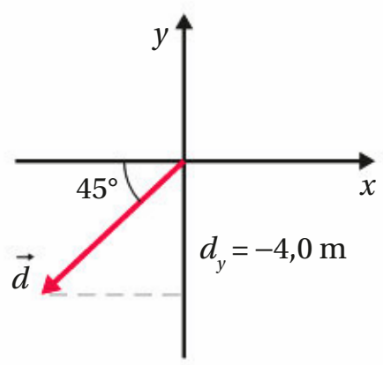
\includegraphics[scale=0.35]{vettored.png}   \end{center} \end{figure}\\
{$A$}: 5,7 m; 4,0 m\ \ {$B$}: -5,7 m; -4,0 m\ \ {$C$}: 5,7 m; -4,0 m\ \ {$D$}: -5,7 m; 4,0 m\ \ 

\mcquestionfooter



\def\mcquestionnumber{10}


\mcquestionheader In quale anno il COVID ha fatto la sua comparsa?\\
{$A$}: 2001\ \ {$B$}: 2019\ \ {$C$}: 1943\ \ {$D$}: 2020\ \ 

\mcquestionfooter



\def\mcquestionnumber{11}


\mcquestionheader I due vettori $\vec{a}$ e $\vec{b}$ hanno lo stesso modulo e la stessa direzione. Quale delle seguenti affermazioni è falsa?\\
{$A$}: La loro somma è sicuramente nulla\ \ {$B$}: Tutte le altre\ \ {$C$}: La loro somma non può mai essere zero\ \ {$D$}: I due vettori sono sicuramente uguali\ \ 

\mcquestionfooter



\def\mcquestionnumber{12}


\mcquestionheader Se mischio blu e giallo che colore ottengo?\\
{$A$}: Giallu\ \ {$B$}: Rosso\ \ {$C$}: Verde\ \ {$D$}: Blallo\ \ 

\mcquestionfooter



\mcpaperfooter

\def\mcserialnumber{29}
\mcpaperheader


\def\mcquestionnumber{1}


\mcquestionheader In quale anno il COVID ha fatto la sua comparsa?\\
{$A$}: 2020\ \ {$B$}: 2019\ \ {$C$}: 1943\ \ {$D$}: 2001\ \ 

\mcquestionfooter



\def\mcquestionnumber{2}


\mcquestionheader Qual è la capitale d’Italia?\\
{$A$}: Roma\ \ {$B$}: Milano\ \ {$C$}: Parigi\ \ {$D$}: Berlino\ \ 

\mcquestionfooter



\def\mcquestionnumber{3}


\mcquestionheader Un gatto percorre 90,0~m verso sud e poi prosegue per altri 120~m verso ovest. Lo spostamento e la distanza percorsa sono rispettivamente\\
{$A$}: 210~m e 210~m\ \ {$B$}: 30~m e 210~m\ \ {$C$}: 150~m e 210~m\ \ {$D$}: 210~m e 150~m\ \ 

\mcquestionfooter



\def\mcquestionnumber{4}


\mcquestionheader Il modulo del vettore $\vec{A}(2;2)$ è\\
{$A$}: non so\ \ {$B$}: chissà\ \ {$C$}: boh\ \ 

\mcquestionfooter



\def\mcquestionnumber{5}


\mcquestionheader In che anno pare sia nato Gesù?\\
{$A$}: 2019\ \ {$B$}: -80\ \ {$C$}: 0\ \ {$D$}: 20\ \ 

\mcquestionfooter



\def\mcquestionnumber{6}


\mcquestionheader Dato il vettore $\vec{d}$ in figura, determina il modulo e la componente $d_x$: \begin{figure}[h!]   \begin{center}     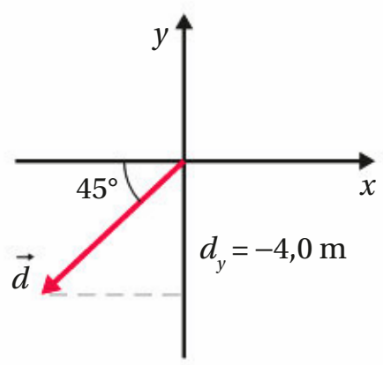
\includegraphics[scale=0.35]{vettored.png}   \end{center} \end{figure}\\
{$A$}: -5,7 m; 4,0 m\ \ {$B$}: -5,7 m; -4,0 m\ \ {$C$}: 5,7 m; -4,0 m\ \ {$D$}: 5,7 m; 4,0 m\ \ 

\mcquestionfooter



\def\mcquestionnumber{7}


\mcquestionheader Raddoppiando la distanza tra due cariche elettriche puntiformi, la forza elettrostatica diminuisce del\\
{$A$}: 90\%\ \ {$B$}: 25\%\ \ {$C$}: 50\%\ \ {$D$}: 75\%\ \ 

\mcquestionfooter



\def\mcquestionnumber{8}


\mcquestionheader I due vettori $\vec{a}$ e $\vec{b}$ hanno lo stesso modulo e la stessa direzione. Quale delle seguenti affermazioni è falsa?\\
{$A$}: I due vettori sono sicuramente uguali\ \ {$B$}: La loro somma è sicuramente nulla\ \ {$C$}: Tutte le altre\ \ {$D$}: La loro somma non può mai essere zero\ \ 

\mcquestionfooter



\def\mcquestionnumber{9}


\mcquestionheader Seguendo la mappa di un tesoro, un pirata cammina per 2,00~km verso nord-est, poi per 5,00~km verso est, quindi per 2,00~km verso sud-est e infine per 3,00~km verso ovest. Arrivato alla fine del percorso a che distanza si trova dalla posizione che occupava alla partenza?\\
{$A$}: 4,76 km\ \ {$B$}: 6,32 km\ \ {$C$}: 4,83 km\ \ {$D$}: 4,59 km\ \ 

\mcquestionfooter



\def\mcquestionnumber{10}


\mcquestionheader Se mischio blu e giallo che colore ottengo?\\
{$A$}: Giallu\ \ {$B$}: Rosso\ \ {$C$}: Verde\ \ {$D$}: Blallo\ \ 

\mcquestionfooter



\def\mcquestionnumber{11}


\mcquestionheader Di che colore era il cavallo bianco di Napoleone?\\
{$A$}: Marrone\ \ {$B$}: Verde\ \ {$C$}: Blu\ \ {$D$}: Bianco\ \ 

\mcquestionfooter



\def\mcquestionnumber{12}


\mcquestionheader Come si chiama il satellite naturale della Terra?\\
{$A$}: Marte\ \ {$B$}: Sole\ \ {$C$}: ISS\ \ {$D$}: Luna\ \ 

\mcquestionfooter



\mcpaperfooter

\def\mcserialnumber{30}
\mcpaperheader


\def\mcquestionnumber{1}


\mcquestionheader Dato il vettore $\vec{d}$ in figura, determina il modulo e la componente $d_x$: \begin{figure}[h!]   \begin{center}     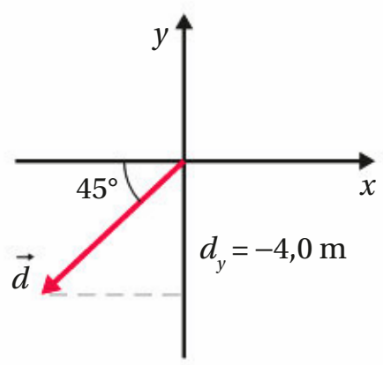
\includegraphics[scale=0.35]{vettored.png}   \end{center} \end{figure}\\
{$A$}: 5,7 m; -4,0 m\ \ {$B$}: -5,7 m; 4,0 m\ \ {$C$}: 5,7 m; 4,0 m\ \ {$D$}: -5,7 m; -4,0 m\ \ 

\mcquestionfooter



\def\mcquestionnumber{2}


\mcquestionheader Seguendo la mappa di un tesoro, un pirata cammina per 2,00~km verso nord-est, poi per 5,00~km verso est, quindi per 2,00~km verso sud-est e infine per 3,00~km verso ovest. Arrivato alla fine del percorso a che distanza si trova dalla posizione che occupava alla partenza?\\
{$A$}: 4,59 km\ \ {$B$}: 4,76 km\ \ {$C$}: 6,32 km\ \ {$D$}: 4,83 km\ \ 

\mcquestionfooter



\def\mcquestionnumber{3}


\mcquestionheader Qual è la capitale d’Italia?\\
{$A$}: Milano\ \ {$B$}: Berlino\ \ {$C$}: Roma\ \ {$D$}: Parigi\ \ 

\mcquestionfooter



\def\mcquestionnumber{4}


\mcquestionheader I due vettori $\vec{a}$ e $\vec{b}$ hanno lo stesso modulo e la stessa direzione. Quale delle seguenti affermazioni è falsa?\\
{$A$}: La loro somma è sicuramente nulla\ \ {$B$}: Tutte le altre\ \ {$C$}: La loro somma non può mai essere zero\ \ {$D$}: I due vettori sono sicuramente uguali\ \ 

\mcquestionfooter



\def\mcquestionnumber{5}


\mcquestionheader Raddoppiando la distanza tra due cariche elettriche puntiformi, la forza elettrostatica diminuisce del\\
{$A$}: 90\%\ \ {$B$}: 75\%\ \ {$C$}: 25\%\ \ {$D$}: 50\%\ \ 

\mcquestionfooter



\def\mcquestionnumber{6}


\mcquestionheader Il modulo del vettore $\vec{A}(3;4)$ è\\
{$A$}: 12\ \ {$B$}: 8\ \ {$C$}: 5\ \ 

\mcquestionfooter



\def\mcquestionnumber{7}


\mcquestionheader In che anno pare sia nato Gesù?\\
{$A$}: 0\ \ {$B$}: 2019\ \ {$C$}: -80\ \ {$D$}: 20\ \ 

\mcquestionfooter



\def\mcquestionnumber{8}


\mcquestionheader Di che colore era il cavallo bianco di Napoleone?\\
{$A$}: Verde\ \ {$B$}: Blu\ \ {$C$}: Marrone\ \ {$D$}: Bianco\ \ 

\mcquestionfooter



\def\mcquestionnumber{9}


\mcquestionheader In quale anno il COVID ha fatto la sua comparsa?\\
{$A$}: 1943\ \ {$B$}: 2020\ \ {$C$}: 2019\ \ {$D$}: 2001\ \ 

\mcquestionfooter



\def\mcquestionnumber{10}


\mcquestionheader Come si chiama il satellite naturale della Terra?\\
{$A$}: Marte\ \ {$B$}: Sole\ \ {$C$}: Luna\ \ {$D$}: ISS\ \ 

\mcquestionfooter



\def\mcquestionnumber{11}


\mcquestionheader Un gatto percorre 90,0~m verso sud e poi prosegue per altri 120~m verso ovest. Lo spostamento e la distanza percorsa sono rispettivamente\\
{$A$}: 150~m e 210~m\ \ {$B$}: 210~m e 150~m\ \ {$C$}: 210~m e 210~m\ \ {$D$}: 30~m e 210~m\ \ 

\mcquestionfooter



\def\mcquestionnumber{12}


\mcquestionheader Se mischio blu e giallo che colore ottengo?\\
{$A$}: Blallo\ \ {$B$}: Rosso\ \ {$C$}: Verde\ \ {$D$}: Giallu\ \ 

\mcquestionfooter



\mcpaperfooter

\def\mcserialnumber{31}
\mcpaperheader


\def\mcquestionnumber{1}


\mcquestionheader Qual è la capitale d’Italia?\\
{$A$}: Berlino\ \ {$B$}: Roma\ \ {$C$}: Parigi\ \ {$D$}: Milano\ \ 

\mcquestionfooter



\def\mcquestionnumber{2}


\mcquestionheader In quale anno il COVID ha fatto la sua comparsa?\\
{$A$}: 1943\ \ {$B$}: 2019\ \ {$C$}: 2001\ \ {$D$}: 2020\ \ 

\mcquestionfooter



\def\mcquestionnumber{3}


\mcquestionheader Di che colore era il cavallo bianco di Napoleone?\\
{$A$}: Marrone\ \ {$B$}: Bianco\ \ {$C$}: Verde\ \ {$D$}: Blu\ \ 

\mcquestionfooter



\def\mcquestionnumber{4}


\mcquestionheader In che anno pare sia nato Gesù?\\
{$A$}: 2019\ \ {$B$}: -80\ \ {$C$}: 0\ \ {$D$}: 20\ \ 

\mcquestionfooter



\def\mcquestionnumber{5}


\mcquestionheader Se mischio blu e giallo che colore ottengo?\\
{$A$}: Verde\ \ {$B$}: Giallu\ \ {$C$}: Rosso\ \ {$D$}: Blallo\ \ 

\mcquestionfooter



\def\mcquestionnumber{6}


\mcquestionheader Dato il vettore $\vec{d}$ in figura, determina il modulo e la componente $d_x$: \begin{figure}[h!]   \begin{center}     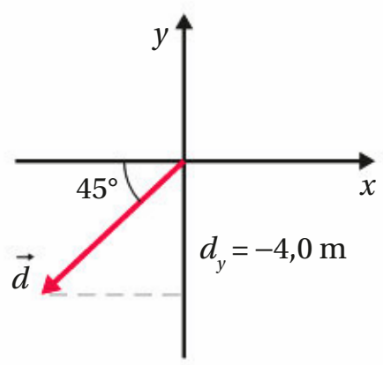
\includegraphics[scale=0.35]{vettored.png}   \end{center} \end{figure}\\
{$A$}: 5,7 m; 4,0 m\ \ {$B$}: -5,7 m; 4,0 m\ \ {$C$}: 5,7 m; -4,0 m\ \ {$D$}: -5,7 m; -4,0 m\ \ 

\mcquestionfooter



\def\mcquestionnumber{7}


\mcquestionheader Seguendo la mappa di un tesoro, un pirata cammina per 2,00~km verso nord-est, poi per 5,00~km verso est, quindi per 2,00~km verso sud-est e infine per 3,00~km verso ovest. Arrivato alla fine del percorso a che distanza si trova dalla posizione che occupava alla partenza?\\
{$A$}: 6,32 km\ \ {$B$}: 4,83 km\ \ {$C$}: 4,59 km\ \ {$D$}: 4,76 km\ \ 

\mcquestionfooter



\def\mcquestionnumber{8}


\mcquestionheader Come si chiama il satellite naturale della Terra?\\
{$A$}: Sole\ \ {$B$}: ISS\ \ {$C$}: Marte\ \ {$D$}: Luna\ \ 

\mcquestionfooter



\def\mcquestionnumber{9}


\mcquestionheader Un gatto percorre 90,0~m verso sud e poi prosegue per altri 120~m verso ovest. Lo spostamento e la distanza percorsa sono rispettivamente\\
{$A$}: 210~m e 150~m\ \ {$B$}: 210~m e 210~m\ \ {$C$}: 30~m e 210~m\ \ {$D$}: 150~m e 210~m\ \ 

\mcquestionfooter



\def\mcquestionnumber{10}


\mcquestionheader Il modulo del vettore $\vec{A}(2;2)$ è\\
{$A$}: chissà\ \ {$B$}: non so\ \ {$C$}: boh\ \ 

\mcquestionfooter



\def\mcquestionnumber{11}


\mcquestionheader I due vettori $\vec{a}$ e $\vec{b}$ hanno lo stesso modulo e la stessa direzione. Quale delle seguenti affermazioni è falsa?\\
{$A$}: La loro somma non può mai essere zero\ \ {$B$}: La loro somma è sicuramente nulla\ \ {$C$}: Tutte le altre\ \ {$D$}: I due vettori sono sicuramente uguali\ \ 

\mcquestionfooter



\def\mcquestionnumber{12}


\mcquestionheader Raddoppiando la distanza tra due cariche elettriche puntiformi, la forza elettrostatica diminuisce del\\
{$A$}: 50\%\ \ {$B$}: 90\%\ \ {$C$}: 75\%\ \ {$D$}: 25\%\ \ 

\mcquestionfooter



\mcpaperfooter

\def\mcserialnumber{32}
\mcpaperheader


\def\mcquestionnumber{1}


\mcquestionheader Se mischio blu e giallo che colore ottengo?\\
{$A$}: Blallo\ \ {$B$}: Verde\ \ {$C$}: Giallu\ \ {$D$}: Rosso\ \ 

\mcquestionfooter



\def\mcquestionnumber{2}


\mcquestionheader Un gatto percorre 90,0~m verso sud e poi prosegue per altri 120~m verso ovest. Lo spostamento e la distanza percorsa sono rispettivamente\\
{$A$}: 210~m e 150~m\ \ {$B$}: 30~m e 210~m\ \ {$C$}: 150~m e 210~m\ \ {$D$}: 210~m e 210~m\ \ 

\mcquestionfooter



\def\mcquestionnumber{3}


\mcquestionheader Di che colore era il cavallo bianco di Napoleone?\\
{$A$}: Bianco\ \ {$B$}: Verde\ \ {$C$}: Marrone\ \ {$D$}: Blu\ \ 

\mcquestionfooter



\def\mcquestionnumber{4}


\mcquestionheader Come si chiama il satellite naturale della Terra?\\
{$A$}: Luna\ \ {$B$}: Marte\ \ {$C$}: ISS\ \ {$D$}: Sole\ \ 

\mcquestionfooter



\def\mcquestionnumber{5}


\mcquestionheader In che anno pare sia nato Gesù?\\
{$A$}: 2019\ \ {$B$}: -80\ \ {$C$}: 20\ \ {$D$}: 0\ \ 

\mcquestionfooter



\def\mcquestionnumber{6}


\mcquestionheader Raddoppiando la distanza tra due cariche elettriche puntiformi, la forza elettrostatica diminuisce del\\
{$A$}: 90\%\ \ {$B$}: 25\%\ \ {$C$}: 75\%\ \ {$D$}: 50\%\ \ 

\mcquestionfooter



\def\mcquestionnumber{7}


\mcquestionheader In quale anno il COVID ha fatto la sua comparsa?\\
{$A$}: 2020\ \ {$B$}: 1943\ \ {$C$}: 2019\ \ {$D$}: 2001\ \ 

\mcquestionfooter



\def\mcquestionnumber{8}


\mcquestionheader Seguendo la mappa di un tesoro, un pirata cammina per 2,00~km verso nord-est, poi per 5,00~km verso est, quindi per 2,00~km verso sud-est e infine per 3,00~km verso ovest. Arrivato alla fine del percorso a che distanza si trova dalla posizione che occupava alla partenza?\\
{$A$}: 6,32 km\ \ {$B$}: 4,59 km\ \ {$C$}: 4,83 km\ \ {$D$}: 4,76 km\ \ 

\mcquestionfooter



\def\mcquestionnumber{9}


\mcquestionheader Il modulo del vettore $\vec{A}(3;4)$ è\\
{$A$}: 8\ \ {$B$}: 5\ \ {$C$}: 12\ \ 

\mcquestionfooter



\def\mcquestionnumber{10}


\mcquestionheader Qual è la capitale d’Italia?\\
{$A$}: Berlino\ \ {$B$}: Milano\ \ {$C$}: Roma\ \ {$D$}: Parigi\ \ 

\mcquestionfooter



\def\mcquestionnumber{11}


\mcquestionheader Dato il vettore $\vec{d}$ in figura, determina il modulo e la componente $d_x$: \begin{figure}[h!]   \begin{center}     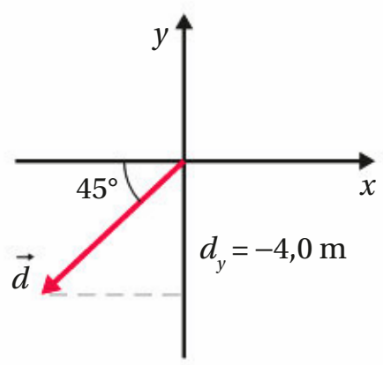
\includegraphics[scale=0.35]{vettored.png}   \end{center} \end{figure}\\
{$A$}: 5,7 m; 4,0 m\ \ {$B$}: -5,7 m; 4,0 m\ \ {$C$}: -5,7 m; -4,0 m\ \ {$D$}: 5,7 m; -4,0 m\ \ 

\mcquestionfooter



\def\mcquestionnumber{12}


\mcquestionheader I due vettori $\vec{a}$ e $\vec{b}$ hanno lo stesso modulo e la stessa direzione. Quale delle seguenti affermazioni è falsa?\\
{$A$}: I due vettori sono sicuramente uguali\ \ {$B$}: La loro somma non può mai essere zero\ \ {$C$}: Tutte le altre\ \ {$D$}: La loro somma è sicuramente nulla\ \ 

\mcquestionfooter



\mcpaperfooter

\def\mcserialnumber{33}
\mcpaperheader


\def\mcquestionnumber{1}


\mcquestionheader Raddoppiando la distanza tra due cariche elettriche puntiformi, la forza elettrostatica diminuisce del\\
{$A$}: 75\%\ \ {$B$}: 90\%\ \ {$C$}: 25\%\ \ {$D$}: 50\%\ \ 

\mcquestionfooter



\def\mcquestionnumber{2}


\mcquestionheader In quale anno il COVID ha fatto la sua comparsa?\\
{$A$}: 2020\ \ {$B$}: 2001\ \ {$C$}: 2019\ \ {$D$}: 1943\ \ 

\mcquestionfooter



\def\mcquestionnumber{3}


\mcquestionheader Un gatto percorre 90,0~m verso sud e poi prosegue per altri 120~m verso ovest. Lo spostamento e la distanza percorsa sono rispettivamente\\
{$A$}: 210~m e 210~m\ \ {$B$}: 210~m e 150~m\ \ {$C$}: 150~m e 210~m\ \ {$D$}: 30~m e 210~m\ \ 

\mcquestionfooter



\def\mcquestionnumber{4}


\mcquestionheader Dato il vettore $\vec{d}$ in figura, determina il modulo e la componente $d_x$: \begin{figure}[h!]   \begin{center}     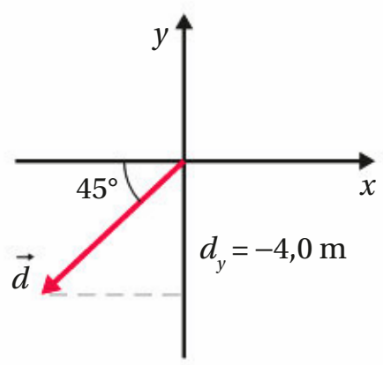
\includegraphics[scale=0.35]{vettored.png}   \end{center} \end{figure}\\
{$A$}: 5,7 m; -4,0 m\ \ {$B$}: 5,7 m; 4,0 m\ \ {$C$}: -5,7 m; -4,0 m\ \ {$D$}: -5,7 m; 4,0 m\ \ 

\mcquestionfooter



\def\mcquestionnumber{5}


\mcquestionheader In che anno pare sia nato Gesù?\\
{$A$}: 0\ \ {$B$}: -80\ \ {$C$}: 20\ \ {$D$}: 2019\ \ 

\mcquestionfooter



\def\mcquestionnumber{6}


\mcquestionheader Il modulo del vettore $\vec{A}(2;2)$ è\\
{$A$}: chissà\ \ {$B$}: boh\ \ {$C$}: non so\ \ 

\mcquestionfooter



\def\mcquestionnumber{7}


\mcquestionheader Di che colore era il cavallo bianco di Napoleone?\\
{$A$}: Verde\ \ {$B$}: Marrone\ \ {$C$}: Bianco\ \ {$D$}: Blu\ \ 

\mcquestionfooter



\def\mcquestionnumber{8}


\mcquestionheader Qual è la capitale d’Italia?\\
{$A$}: Milano\ \ {$B$}: Parigi\ \ {$C$}: Roma\ \ {$D$}: Berlino\ \ 

\mcquestionfooter



\def\mcquestionnumber{9}


\mcquestionheader Come si chiama il satellite naturale della Terra?\\
{$A$}: Sole\ \ {$B$}: Luna\ \ {$C$}: ISS\ \ {$D$}: Marte\ \ 

\mcquestionfooter



\def\mcquestionnumber{10}


\mcquestionheader I due vettori $\vec{a}$ e $\vec{b}$ hanno lo stesso modulo e la stessa direzione. Quale delle seguenti affermazioni è falsa?\\
{$A$}: Tutte le altre\ \ {$B$}: La loro somma non può mai essere zero\ \ {$C$}: I due vettori sono sicuramente uguali\ \ {$D$}: La loro somma è sicuramente nulla\ \ 

\mcquestionfooter



\def\mcquestionnumber{11}


\mcquestionheader Seguendo la mappa di un tesoro, un pirata cammina per 2,00~km verso nord-est, poi per 5,00~km verso est, quindi per 2,00~km verso sud-est e infine per 3,00~km verso ovest. Arrivato alla fine del percorso a che distanza si trova dalla posizione che occupava alla partenza?\\
{$A$}: 4,76 km\ \ {$B$}: 4,59 km\ \ {$C$}: 4,83 km\ \ {$D$}: 6,32 km\ \ 

\mcquestionfooter



\def\mcquestionnumber{12}


\mcquestionheader Se mischio blu e giallo che colore ottengo?\\
{$A$}: Giallu\ \ {$B$}: Blallo\ \ {$C$}: Verde\ \ {$D$}: Rosso\ \ 

\mcquestionfooter



\mcpaperfooter

\def\mcserialnumber{34}
\mcpaperheader


\def\mcquestionnumber{1}


\mcquestionheader Il modulo del vettore $\vec{A}(2;2)$ è\\
{$A$}: chissà\ \ {$B$}: non so\ \ {$C$}: boh\ \ 

\mcquestionfooter



\def\mcquestionnumber{2}


\mcquestionheader Come si chiama il satellite naturale della Terra?\\
{$A$}: Luna\ \ {$B$}: Marte\ \ {$C$}: Sole\ \ {$D$}: ISS\ \ 

\mcquestionfooter



\def\mcquestionnumber{3}


\mcquestionheader Se mischio blu e giallo che colore ottengo?\\
{$A$}: Giallu\ \ {$B$}: Blallo\ \ {$C$}: Verde\ \ {$D$}: Rosso\ \ 

\mcquestionfooter



\def\mcquestionnumber{4}


\mcquestionheader Qual è la capitale d’Italia?\\
{$A$}: Berlino\ \ {$B$}: Milano\ \ {$C$}: Parigi\ \ {$D$}: Roma\ \ 

\mcquestionfooter



\def\mcquestionnumber{5}


\mcquestionheader Raddoppiando la distanza tra due cariche elettriche puntiformi, la forza elettrostatica diminuisce del\\
{$A$}: 90\%\ \ {$B$}: 75\%\ \ {$C$}: 25\%\ \ {$D$}: 50\%\ \ 

\mcquestionfooter



\def\mcquestionnumber{6}


\mcquestionheader Un gatto percorre 90,0~m verso sud e poi prosegue per altri 120~m verso ovest. Lo spostamento e la distanza percorsa sono rispettivamente\\
{$A$}: 210~m e 150~m\ \ {$B$}: 210~m e 210~m\ \ {$C$}: 30~m e 210~m\ \ {$D$}: 150~m e 210~m\ \ 

\mcquestionfooter



\def\mcquestionnumber{7}


\mcquestionheader Di che colore era il cavallo bianco di Napoleone?\\
{$A$}: Bianco\ \ {$B$}: Blu\ \ {$C$}: Verde\ \ {$D$}: Marrone\ \ 

\mcquestionfooter



\def\mcquestionnumber{8}


\mcquestionheader I due vettori $\vec{a}$ e $\vec{b}$ hanno lo stesso modulo e la stessa direzione. Quale delle seguenti affermazioni è falsa?\\
{$A$}: Tutte le altre\ \ {$B$}: La loro somma è sicuramente nulla\ \ {$C$}: La loro somma non può mai essere zero\ \ {$D$}: I due vettori sono sicuramente uguali\ \ 

\mcquestionfooter



\def\mcquestionnumber{9}


\mcquestionheader In che anno pare sia nato Gesù?\\
{$A$}: 0\ \ {$B$}: 20\ \ {$C$}: -80\ \ {$D$}: 2019\ \ 

\mcquestionfooter



\def\mcquestionnumber{10}


\mcquestionheader Dato il vettore $\vec{d}$ in figura, determina il modulo e la componente $d_x$: \begin{figure}[h!]   \begin{center}     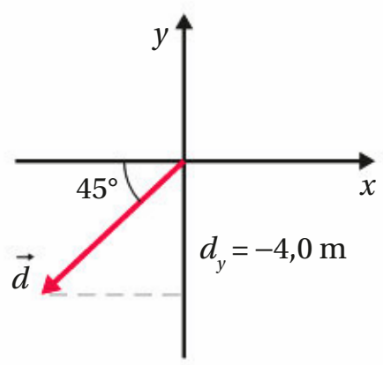
\includegraphics[scale=0.35]{vettored.png}   \end{center} \end{figure}\\
{$A$}: -5,7 m; 4,0 m\ \ {$B$}: 5,7 m; 4,0 m\ \ {$C$}: -5,7 m; -4,0 m\ \ {$D$}: 5,7 m; -4,0 m\ \ 

\mcquestionfooter



\def\mcquestionnumber{11}


\mcquestionheader Seguendo la mappa di un tesoro, un pirata cammina per 2,00~km verso nord-est, poi per 5,00~km verso est, quindi per 2,00~km verso sud-est e infine per 3,00~km verso ovest. Arrivato alla fine del percorso a che distanza si trova dalla posizione che occupava alla partenza?\\
{$A$}: 4,76 km\ \ {$B$}: 6,32 km\ \ {$C$}: 4,59 km\ \ {$D$}: 4,83 km\ \ 

\mcquestionfooter



\def\mcquestionnumber{12}


\mcquestionheader In quale anno il COVID ha fatto la sua comparsa?\\
{$A$}: 2001\ \ {$B$}: 1943\ \ {$C$}: 2019\ \ {$D$}: 2020\ \ 

\mcquestionfooter



\mcpaperfooter

\def\mcserialnumber{35}
\mcpaperheader


\def\mcquestionnumber{1}


\mcquestionheader Qual è la capitale d’Italia?\\
{$A$}: Milano\ \ {$B$}: Roma\ \ {$C$}: Parigi\ \ {$D$}: Berlino\ \ 

\mcquestionfooter



\def\mcquestionnumber{2}


\mcquestionheader Un gatto percorre 90,0~m verso sud e poi prosegue per altri 120~m verso ovest. Lo spostamento e la distanza percorsa sono rispettivamente\\
{$A$}: 150~m e 210~m\ \ {$B$}: 210~m e 210~m\ \ {$C$}: 30~m e 210~m\ \ {$D$}: 210~m e 150~m\ \ 

\mcquestionfooter



\def\mcquestionnumber{3}


\mcquestionheader Se mischio blu e giallo che colore ottengo?\\
{$A$}: Giallu\ \ {$B$}: Rosso\ \ {$C$}: Verde\ \ {$D$}: Blallo\ \ 

\mcquestionfooter



\def\mcquestionnumber{4}


\mcquestionheader Di che colore era il cavallo bianco di Napoleone?\\
{$A$}: Bianco\ \ {$B$}: Blu\ \ {$C$}: Verde\ \ {$D$}: Marrone\ \ 

\mcquestionfooter



\def\mcquestionnumber{5}


\mcquestionheader Raddoppiando la distanza tra due cariche elettriche puntiformi, la forza elettrostatica diminuisce del\\
{$A$}: 90\%\ \ {$B$}: 25\%\ \ {$C$}: 75\%\ \ {$D$}: 50\%\ \ 

\mcquestionfooter



\def\mcquestionnumber{6}


\mcquestionheader Il modulo del vettore $\vec{A}(3;4)$ è\\
{$A$}: 8\ \ {$B$}: 12\ \ {$C$}: 5\ \ 

\mcquestionfooter



\def\mcquestionnumber{7}


\mcquestionheader In quale anno il COVID ha fatto la sua comparsa?\\
{$A$}: 2020\ \ {$B$}: 2001\ \ {$C$}: 1943\ \ {$D$}: 2019\ \ 

\mcquestionfooter



\def\mcquestionnumber{8}


\mcquestionheader In che anno pare sia nato Gesù?\\
{$A$}: -80\ \ {$B$}: 20\ \ {$C$}: 2019\ \ {$D$}: 0\ \ 

\mcquestionfooter



\def\mcquestionnumber{9}


\mcquestionheader I due vettori $\vec{a}$ e $\vec{b}$ hanno lo stesso modulo e la stessa direzione. Quale delle seguenti affermazioni è falsa?\\
{$A$}: La loro somma non può mai essere zero\ \ {$B$}: Tutte le altre\ \ {$C$}: La loro somma è sicuramente nulla\ \ {$D$}: I due vettori sono sicuramente uguali\ \ 

\mcquestionfooter



\def\mcquestionnumber{10}


\mcquestionheader Seguendo la mappa di un tesoro, un pirata cammina per 2,00~km verso nord-est, poi per 5,00~km verso est, quindi per 2,00~km verso sud-est e infine per 3,00~km verso ovest. Arrivato alla fine del percorso a che distanza si trova dalla posizione che occupava alla partenza?\\
{$A$}: 4,59 km\ \ {$B$}: 6,32 km\ \ {$C$}: 4,83 km\ \ {$D$}: 4,76 km\ \ 

\mcquestionfooter



\def\mcquestionnumber{11}


\mcquestionheader Dato il vettore $\vec{d}$ in figura, determina il modulo e la componente $d_x$: \begin{figure}[h!]   \begin{center}     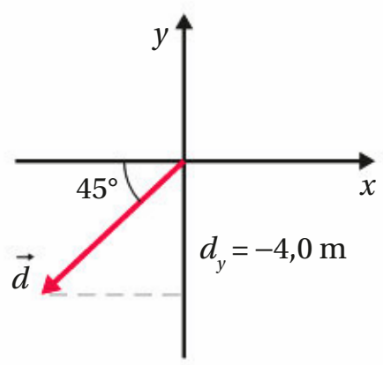
\includegraphics[scale=0.35]{vettored.png}   \end{center} \end{figure}\\
{$A$}: 5,7 m; -4,0 m\ \ {$B$}: -5,7 m; 4,0 m\ \ {$C$}: -5,7 m; -4,0 m\ \ {$D$}: 5,7 m; 4,0 m\ \ 

\mcquestionfooter



\def\mcquestionnumber{12}


\mcquestionheader Come si chiama il satellite naturale della Terra?\\
{$A$}: Marte\ \ {$B$}: Sole\ \ {$C$}: ISS\ \ {$D$}: Luna\ \ 

\mcquestionfooter



\mcpaperfooter

\def\mcserialnumber{36}
\mcpaperheader


\def\mcquestionnumber{1}


\mcquestionheader Qual è la capitale d’Italia?\\
{$A$}: Parigi\ \ {$B$}: Berlino\ \ {$C$}: Roma\ \ {$D$}: Milano\ \ 

\mcquestionfooter



\def\mcquestionnumber{2}


\mcquestionheader Di che colore era il cavallo bianco di Napoleone?\\
{$A$}: Bianco\ \ {$B$}: Blu\ \ {$C$}: Marrone\ \ {$D$}: Verde\ \ 

\mcquestionfooter



\def\mcquestionnumber{3}


\mcquestionheader Il modulo del vettore $\vec{A}(2;2)$ è\\
{$A$}: boh\ \ {$B$}: non so\ \ {$C$}: chissà\ \ 

\mcquestionfooter



\def\mcquestionnumber{4}


\mcquestionheader Dato il vettore $\vec{d}$ in figura, determina il modulo e la componente $d_x$: \begin{figure}[h!]   \begin{center}     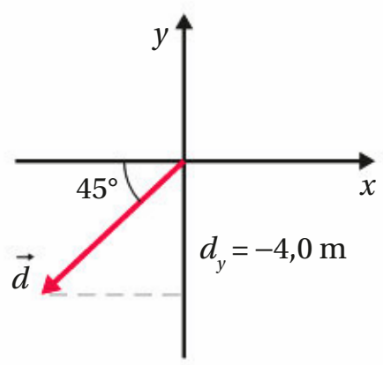
\includegraphics[scale=0.35]{vettored.png}   \end{center} \end{figure}\\
{$A$}: 5,7 m; 4,0 m\ \ {$B$}: -5,7 m; -4,0 m\ \ {$C$}: -5,7 m; 4,0 m\ \ {$D$}: 5,7 m; -4,0 m\ \ 

\mcquestionfooter



\def\mcquestionnumber{5}


\mcquestionheader In quale anno il COVID ha fatto la sua comparsa?\\
{$A$}: 2019\ \ {$B$}: 2020\ \ {$C$}: 1943\ \ {$D$}: 2001\ \ 

\mcquestionfooter



\def\mcquestionnumber{6}


\mcquestionheader Seguendo la mappa di un tesoro, un pirata cammina per 2,00~km verso nord-est, poi per 5,00~km verso est, quindi per 2,00~km verso sud-est e infine per 3,00~km verso ovest. Arrivato alla fine del percorso a che distanza si trova dalla posizione che occupava alla partenza?\\
{$A$}: 4,59 km\ \ {$B$}: 4,83 km\ \ {$C$}: 6,32 km\ \ {$D$}: 4,76 km\ \ 

\mcquestionfooter



\def\mcquestionnumber{7}


\mcquestionheader Raddoppiando la distanza tra due cariche elettriche puntiformi, la forza elettrostatica diminuisce del\\
{$A$}: 75\%\ \ {$B$}: 90\%\ \ {$C$}: 50\%\ \ {$D$}: 25\%\ \ 

\mcquestionfooter



\def\mcquestionnumber{8}


\mcquestionheader Se mischio blu e giallo che colore ottengo?\\
{$A$}: Giallu\ \ {$B$}: Verde\ \ {$C$}: Rosso\ \ {$D$}: Blallo\ \ 

\mcquestionfooter



\def\mcquestionnumber{9}


\mcquestionheader I due vettori $\vec{a}$ e $\vec{b}$ hanno lo stesso modulo e la stessa direzione. Quale delle seguenti affermazioni è falsa?\\
{$A$}: La loro somma non può mai essere zero\ \ {$B$}: Tutte le altre\ \ {$C$}: I due vettori sono sicuramente uguali\ \ {$D$}: La loro somma è sicuramente nulla\ \ 

\mcquestionfooter



\def\mcquestionnumber{10}


\mcquestionheader Come si chiama il satellite naturale della Terra?\\
{$A$}: ISS\ \ {$B$}: Sole\ \ {$C$}: Marte\ \ {$D$}: Luna\ \ 

\mcquestionfooter



\def\mcquestionnumber{11}


\mcquestionheader Un gatto percorre 90,0~m verso sud e poi prosegue per altri 120~m verso ovest. Lo spostamento e la distanza percorsa sono rispettivamente\\
{$A$}: 210~m e 150~m\ \ {$B$}: 150~m e 210~m\ \ {$C$}: 210~m e 210~m\ \ {$D$}: 30~m e 210~m\ \ 

\mcquestionfooter



\def\mcquestionnumber{12}


\mcquestionheader In che anno pare sia nato Gesù?\\
{$A$}: 2019\ \ {$B$}: 20\ \ {$C$}: -80\ \ {$D$}: 0\ \ 

\mcquestionfooter



\mcpaperfooter

\def\mcserialnumber{37}
\mcpaperheader


\def\mcquestionnumber{1}


\mcquestionheader In che anno pare sia nato Gesù?\\
{$A$}: -80\ \ {$B$}: 20\ \ {$C$}: 2019\ \ {$D$}: 0\ \ 

\mcquestionfooter



\def\mcquestionnumber{2}


\mcquestionheader I due vettori $\vec{a}$ e $\vec{b}$ hanno lo stesso modulo e la stessa direzione. Quale delle seguenti affermazioni è falsa?\\
{$A$}: Tutte le altre\ \ {$B$}: La loro somma non può mai essere zero\ \ {$C$}: La loro somma è sicuramente nulla\ \ {$D$}: I due vettori sono sicuramente uguali\ \ 

\mcquestionfooter



\def\mcquestionnumber{3}


\mcquestionheader Dato il vettore $\vec{d}$ in figura, determina il modulo e la componente $d_x$: \begin{figure}[h!]   \begin{center}     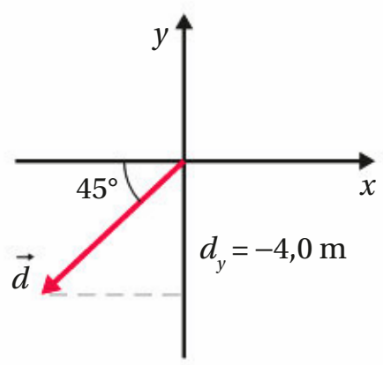
\includegraphics[scale=0.35]{vettored.png}   \end{center} \end{figure}\\
{$A$}: -5,7 m; -4,0 m\ \ {$B$}: 5,7 m; 4,0 m\ \ {$C$}: -5,7 m; 4,0 m\ \ {$D$}: 5,7 m; -4,0 m\ \ 

\mcquestionfooter



\def\mcquestionnumber{4}


\mcquestionheader Il modulo del vettore $\vec{A}(3;4)$ è\\
{$A$}: 12\ \ {$B$}: 8\ \ {$C$}: 5\ \ 

\mcquestionfooter



\def\mcquestionnumber{5}


\mcquestionheader Come si chiama il satellite naturale della Terra?\\
{$A$}: Sole\ \ {$B$}: Luna\ \ {$C$}: ISS\ \ {$D$}: Marte\ \ 

\mcquestionfooter



\def\mcquestionnumber{6}


\mcquestionheader Raddoppiando la distanza tra due cariche elettriche puntiformi, la forza elettrostatica diminuisce del\\
{$A$}: 90\%\ \ {$B$}: 50\%\ \ {$C$}: 25\%\ \ {$D$}: 75\%\ \ 

\mcquestionfooter



\def\mcquestionnumber{7}


\mcquestionheader Seguendo la mappa di un tesoro, un pirata cammina per 2,00~km verso nord-est, poi per 5,00~km verso est, quindi per 2,00~km verso sud-est e infine per 3,00~km verso ovest. Arrivato alla fine del percorso a che distanza si trova dalla posizione che occupava alla partenza?\\
{$A$}: 4,83 km\ \ {$B$}: 6,32 km\ \ {$C$}: 4,76 km\ \ {$D$}: 4,59 km\ \ 

\mcquestionfooter



\def\mcquestionnumber{8}


\mcquestionheader In quale anno il COVID ha fatto la sua comparsa?\\
{$A$}: 2001\ \ {$B$}: 2020\ \ {$C$}: 1943\ \ {$D$}: 2019\ \ 

\mcquestionfooter



\def\mcquestionnumber{9}


\mcquestionheader Se mischio blu e giallo che colore ottengo?\\
{$A$}: Blallo\ \ {$B$}: Giallu\ \ {$C$}: Verde\ \ {$D$}: Rosso\ \ 

\mcquestionfooter



\def\mcquestionnumber{10}


\mcquestionheader Di che colore era il cavallo bianco di Napoleone?\\
{$A$}: Bianco\ \ {$B$}: Marrone\ \ {$C$}: Verde\ \ {$D$}: Blu\ \ 

\mcquestionfooter



\def\mcquestionnumber{11}


\mcquestionheader Qual è la capitale d’Italia?\\
{$A$}: Berlino\ \ {$B$}: Roma\ \ {$C$}: Parigi\ \ {$D$}: Milano\ \ 

\mcquestionfooter



\def\mcquestionnumber{12}


\mcquestionheader Un gatto percorre 90,0~m verso sud e poi prosegue per altri 120~m verso ovest. Lo spostamento e la distanza percorsa sono rispettivamente\\
{$A$}: 210~m e 210~m\ \ {$B$}: 210~m e 150~m\ \ {$C$}: 150~m e 210~m\ \ {$D$}: 30~m e 210~m\ \ 

\mcquestionfooter



\mcpaperfooter

\def\mcserialnumber{38}
\mcpaperheader


\def\mcquestionnumber{1}


\mcquestionheader Il modulo del vettore $\vec{A}(2;2)$ è\\
{$A$}: non so\ \ {$B$}: chissà\ \ {$C$}: boh\ \ 

\mcquestionfooter



\def\mcquestionnumber{2}


\mcquestionheader Un gatto percorre 90,0~m verso sud e poi prosegue per altri 120~m verso ovest. Lo spostamento e la distanza percorsa sono rispettivamente\\
{$A$}: 30~m e 210~m\ \ {$B$}: 150~m e 210~m\ \ {$C$}: 210~m e 210~m\ \ {$D$}: 210~m e 150~m\ \ 

\mcquestionfooter



\def\mcquestionnumber{3}


\mcquestionheader Di che colore era il cavallo bianco di Napoleone?\\
{$A$}: Marrone\ \ {$B$}: Verde\ \ {$C$}: Blu\ \ {$D$}: Bianco\ \ 

\mcquestionfooter



\def\mcquestionnumber{4}


\mcquestionheader Qual è la capitale d’Italia?\\
{$A$}: Berlino\ \ {$B$}: Roma\ \ {$C$}: Milano\ \ {$D$}: Parigi\ \ 

\mcquestionfooter



\def\mcquestionnumber{5}


\mcquestionheader I due vettori $\vec{a}$ e $\vec{b}$ hanno lo stesso modulo e la stessa direzione. Quale delle seguenti affermazioni è falsa?\\
{$A$}: Tutte le altre\ \ {$B$}: I due vettori sono sicuramente uguali\ \ {$C$}: La loro somma non può mai essere zero\ \ {$D$}: La loro somma è sicuramente nulla\ \ 

\mcquestionfooter



\def\mcquestionnumber{6}


\mcquestionheader In quale anno il COVID ha fatto la sua comparsa?\\
{$A$}: 2020\ \ {$B$}: 1943\ \ {$C$}: 2001\ \ {$D$}: 2019\ \ 

\mcquestionfooter



\def\mcquestionnumber{7}


\mcquestionheader In che anno pare sia nato Gesù?\\
{$A$}: 0\ \ {$B$}: 2019\ \ {$C$}: 20\ \ {$D$}: -80\ \ 

\mcquestionfooter



\def\mcquestionnumber{8}


\mcquestionheader Seguendo la mappa di un tesoro, un pirata cammina per 2,00~km verso nord-est, poi per 5,00~km verso est, quindi per 2,00~km verso sud-est e infine per 3,00~km verso ovest. Arrivato alla fine del percorso a che distanza si trova dalla posizione che occupava alla partenza?\\
{$A$}: 4,83 km\ \ {$B$}: 4,76 km\ \ {$C$}: 6,32 km\ \ {$D$}: 4,59 km\ \ 

\mcquestionfooter



\def\mcquestionnumber{9}


\mcquestionheader Raddoppiando la distanza tra due cariche elettriche puntiformi, la forza elettrostatica diminuisce del\\
{$A$}: 90\%\ \ {$B$}: 75\%\ \ {$C$}: 25\%\ \ {$D$}: 50\%\ \ 

\mcquestionfooter



\def\mcquestionnumber{10}


\mcquestionheader Se mischio blu e giallo che colore ottengo?\\
{$A$}: Verde\ \ {$B$}: Rosso\ \ {$C$}: Blallo\ \ {$D$}: Giallu\ \ 

\mcquestionfooter



\def\mcquestionnumber{11}


\mcquestionheader Come si chiama il satellite naturale della Terra?\\
{$A$}: ISS\ \ {$B$}: Luna\ \ {$C$}: Marte\ \ {$D$}: Sole\ \ 

\mcquestionfooter



\def\mcquestionnumber{12}


\mcquestionheader Dato il vettore $\vec{d}$ in figura, determina il modulo e la componente $d_x$: \begin{figure}[h!]   \begin{center}     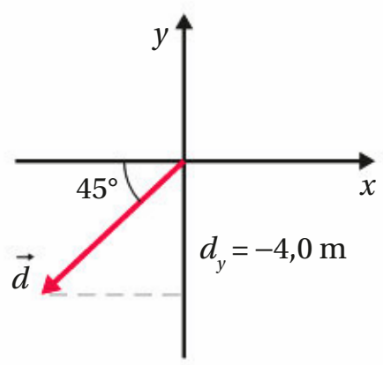
\includegraphics[scale=0.35]{vettored.png}   \end{center} \end{figure}\\
{$A$}: 5,7 m; -4,0 m\ \ {$B$}: 5,7 m; 4,0 m\ \ {$C$}: -5,7 m; 4,0 m\ \ {$D$}: -5,7 m; -4,0 m\ \ 

\mcquestionfooter



\mcpaperfooter

\def\mcserialnumber{39}
\mcpaperheader


\def\mcquestionnumber{1}


\mcquestionheader Seguendo la mappa di un tesoro, un pirata cammina per 2,00~km verso nord-est, poi per 5,00~km verso est, quindi per 2,00~km verso sud-est e infine per 3,00~km verso ovest. Arrivato alla fine del percorso a che distanza si trova dalla posizione che occupava alla partenza?\\
{$A$}: 4,83 km\ \ {$B$}: 4,59 km\ \ {$C$}: 4,76 km\ \ {$D$}: 6,32 km\ \ 

\mcquestionfooter



\def\mcquestionnumber{2}


\mcquestionheader Come si chiama il satellite naturale della Terra?\\
{$A$}: Sole\ \ {$B$}: ISS\ \ {$C$}: Marte\ \ {$D$}: Luna\ \ 

\mcquestionfooter



\def\mcquestionnumber{3}


\mcquestionheader Di che colore era il cavallo bianco di Napoleone?\\
{$A$}: Verde\ \ {$B$}: Marrone\ \ {$C$}: Bianco\ \ {$D$}: Blu\ \ 

\mcquestionfooter



\def\mcquestionnumber{4}


\mcquestionheader Un gatto percorre 90,0~m verso sud e poi prosegue per altri 120~m verso ovest. Lo spostamento e la distanza percorsa sono rispettivamente\\
{$A$}: 210~m e 210~m\ \ {$B$}: 30~m e 210~m\ \ {$C$}: 150~m e 210~m\ \ {$D$}: 210~m e 150~m\ \ 

\mcquestionfooter



\def\mcquestionnumber{5}


\mcquestionheader Qual è la capitale d’Italia?\\
{$A$}: Milano\ \ {$B$}: Roma\ \ {$C$}: Berlino\ \ {$D$}: Parigi\ \ 

\mcquestionfooter



\def\mcquestionnumber{6}


\mcquestionheader Dato il vettore $\vec{d}$ in figura, determina il modulo e la componente $d_x$: \begin{figure}[h!]   \begin{center}     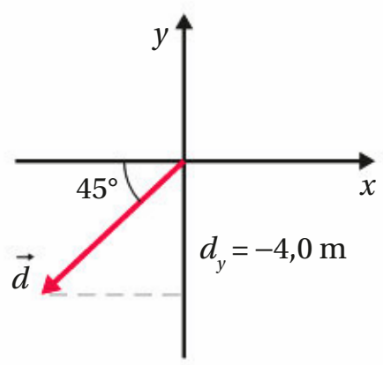
\includegraphics[scale=0.35]{vettored.png}   \end{center} \end{figure}\\
{$A$}: 5,7 m; -4,0 m\ \ {$B$}: -5,7 m; 4,0 m\ \ {$C$}: -5,7 m; -4,0 m\ \ {$D$}: 5,7 m; 4,0 m\ \ 

\mcquestionfooter



\def\mcquestionnumber{7}


\mcquestionheader Raddoppiando la distanza tra due cariche elettriche puntiformi, la forza elettrostatica diminuisce del\\
{$A$}: 90\%\ \ {$B$}: 75\%\ \ {$C$}: 25\%\ \ {$D$}: 50\%\ \ 

\mcquestionfooter



\def\mcquestionnumber{8}


\mcquestionheader In che anno pare sia nato Gesù?\\
{$A$}: -80\ \ {$B$}: 2019\ \ {$C$}: 0\ \ {$D$}: 20\ \ 

\mcquestionfooter



\def\mcquestionnumber{9}


\mcquestionheader I due vettori $\vec{a}$ e $\vec{b}$ hanno lo stesso modulo e la stessa direzione. Quale delle seguenti affermazioni è falsa?\\
{$A$}: La loro somma non può mai essere zero\ \ {$B$}: I due vettori sono sicuramente uguali\ \ {$C$}: La loro somma è sicuramente nulla\ \ {$D$}: Tutte le altre\ \ 

\mcquestionfooter



\def\mcquestionnumber{10}


\mcquestionheader Se mischio blu e giallo che colore ottengo?\\
{$A$}: Giallu\ \ {$B$}: Blallo\ \ {$C$}: Verde\ \ {$D$}: Rosso\ \ 

\mcquestionfooter



\def\mcquestionnumber{11}


\mcquestionheader In quale anno il COVID ha fatto la sua comparsa?\\
{$A$}: 1943\ \ {$B$}: 2001\ \ {$C$}: 2020\ \ {$D$}: 2019\ \ 

\mcquestionfooter



\def\mcquestionnumber{12}


\mcquestionheader Il modulo del vettore $\vec{A}(2;2)$ è\\
{$A$}: non so\ \ {$B$}: boh\ \ {$C$}: chissà\ \ 

\mcquestionfooter



\mcpaperfooter

